%yright 2007, 2008, 2009 Elsevier Ltd
%% 
%% This file is part of the 'Elsarticle Bundle'.
%% ---------------------------------------------
%% 
%% It may be distributed under the conditions of the LaTeX Project Public
%% License, either version 1.2 of this license or (at your option) any
%% later version.  The latest version of this license is in
%%    http://www.latex-project.org/lppl.txt
%% and version 1.2 or later is part of all distributions of LaTeX
%% version 1999/12/01 or later.
%% 
%% The list of all files belonging to the 'Elsarticle Bundle' is
%% given in the file `manifest.txt'.
%% 

%% Template article for Elsevier's document class `elsarticle'
%% with numbered style bibliographic references
%% SP 2008/03/01

% \documentclass[preprint,11pt]{elsarticle}
\documentclass[final,1p,11pt]{elsarticle}

%\documentclass[final,1p,times]{elsarticle}


%% Use the option review to obtain double line spacing
%%\documentclass[authoryear,preprint,review,12pt]{elsarticle}

%% Use the options 1p,twocolumn; 3p; 3p,twocolumn; 5p; or 5p,twocolumn
%% for a journal layout:
%% \documentclass[final,1p,times]{elsarticle}
%% \documentclass[final,1p,times,twocolumn]{elsarticle}
%% \documentclass[final,3p,times]{elsarticle}
%% \documentclass[final,3p,times,twocolumn]{elsarticle}
%% \documentclass[final,5p,times]{elsarticle}
%% \documentclass[final,5p,times,twocolumn]{elsarticle}

%%% For including figures, graphicx.sty has been loaded in
%% elsarticle.cls. If you prefer to use the old commands
%% please give \usepackage{epsfig}


\usepackage{epsfig}
%\usepackage{cite}
%\usepackage{mcite}
\usepackage{array,tabularx,epsfig,mathrsfs,graphicx,rotating}
\usepackage{ifthen}
\usepackage{amsfonts}
\usepackage{ragged2e}
\PassOptionsToPackage{hyphens}{url}
\usepackage[hyphens]{url}
\usepackage{hyperref}
\usepackage{listings}
\usepackage{subfigure}
\usepackage{epstopdf}
% Custom colors
\usepackage{color}
\usepackage{float}

% to cross text
\usepackage[normalem]{ulem} % either use this (simple) or
\usepackage{soul} % use this (many fancier options)


\hypersetup{
  colorlinks=true,
  linkcolor=blue,
  citecolor=blue,
  urlcolor=blue
}




\graphicspath{{figs/}}


\pdfinfo{
   /Author (Chekanov/Demarteau)
   /Title  (Conceptual Design Studies for a CEPC Detector)
   /CreationDate (D:20160102195600)
   /Subject (PDFLaTeX)
   /Keywords (PDF;LaTeX)
}


\textheight=22cm
\textwidth=14.5cm

\newcommand{\beq}{\begin{equation}}
\newcommand{\eeq}{\end{equation}}
\newcommand{\la}{\langle}
\newcommand{\promc}{{\sc ProMC}}
\newcommand{\ra}{\rangle}
\newcommand{\eps}{\epsilon}
\newcommand{\ud}{\mathrm{d}}
\newcommand{\Ec}{\mathcal{E}}
\newcommand{\Fc}{\mathcal{F}}
\newcommand{\Za}{\mathrm{Z_1}}
\newcommand{\Zb}{\mathrm{Z_2}}
\newcommand{\Zn}{\mathrm{Z_n}}
\newcommand{\F}{\mathrm{F}}

\chardef\til=126
\newcommand{\mev}{{\,\mathrm{MeV}}}
\newcommand{\gev}{{\,\mathrm{GeV}}}
\newcommand{\tev}{{\,\mathrm{TeV}}}
\newcommand{\GEANTfour} {\textsc{geant4}}
\journal{XXX-XXX}



\begin{document}

\definecolor{mygreen}{rgb}{0,0.6,0} \definecolor{mygray}{rgb}{0.5,0.5,0.5} \definecolor{mymauve}{rgb}{0.58,0,0.82}

\lstset{ %
 backgroundcolor=\color{white},   % choose the background color; you must add \usepackage{color} or \usepackage{xcolor}
 basicstyle=\footnotesize,        % the size of the fonts that are used for the code
 breakatwhitespace=false,         % sets if automatic breaks should only happen at whitespace
 breaklines=true,                 % sets automatic line breaking
 captionpos=b,                    % sets the caption-position to bottom
 commentstyle=\color{mygreen},    % comment style
 deletekeywords={...},            % if you want to delete keywords from the given language
 escapeinside={\%*}{*)},          % if you want to add LaTeX within your code
 extendedchars=true,              % lets you use non-ASCII characters; for 8-bits encodings only, does not work with UTF-8
 keepspaces=true,                 % keeps spaces in text, useful for keeping indentation of code (possibly needs columns=flexible)
 frame=tb,
 keywordstyle=\color{blue},       % keyword style
 language=Python,                 % the language of the code
 otherkeywords={*,...},            % if you want to add more keywords to the set
 rulecolor=\color{black},         % if not set, the frame-color may be changed on line-breaks within not-black text (e.g. comments (green here))
 showspaces=false,                % show spaces everywhere adding particular underscores; it overrides 'showstringspaces'
 showstringspaces=false,          % underline spaces within strings only
 showtabs=false,                  % show tabs within strings adding particular underscores
 stepnumber=2,                    % the step between two line-numbers. If it's 1, each line will be numbered
 stringstyle=\color{mymauve},     % string literal style
 tabsize=2,                        % sets default tabsize to 2 spaces
 title=\lstname,                   % show the filename of files included with \lstinputlisting; also try caption instead of title
 numberstyle=\footnotesize,
 basicstyle=\small,
 basewidth={0.5em,0.5em}
}


\begin{frontmatter}

\title{
Studies of granularity of a hadronic calorimeter for tens-of-TeV jets  at a 100~TeV $pp$ collider 
}
%%%%%%%%%%%%%%%%%%%%%%%%%%%%%%%%%%%%%%%%%%%%%%%%%%%%%%%%%%%%%%%

\author[add1]{S.V.~Chekanov}
\ead{chekanov@anl.gov}

\author[addDuke,add2]{A.V.~Kotwal}
\ead{ashutosh.kotwal@duke.edu}

\author[add1]{J.~Proudfoot}
\ead{proudfoot@anl.gov}

\author[addDuke]{S.~Sen}
\ead{sourav.sen@duke.edu}

\author[add2]{N.V.~Tran}
\ead{ntran@fnal.gov}

\author[add3]{S.-S.~Yu}
\ead{syu@cern.ch}

\author[add3]{Chih-Hsiang Yeh}
\ead{jwzuzelski18@gmail.com}

\address[add1]{
HEP Division, Argonne National Laboratory,
9700 S.~Cass Avenue,
Argonne, IL 60439, USA. 
}

\address[addDuke]{
Department of Physics, Duke University, USA
}

\address[add2]{
Fermi National Accelerator Laboratory
}

\address[addMSU]{
Department of Physics, Michigan State University, 220
Trowbridge Road, East Lansing, MI 48824 
}


\address[add3]{
Department of Physics, National Central University, Chung-Li, Taoyuan City 32001, Taiwan
}


\begin{abstract}
Texts

\end{abstract}

\begin{keyword}
multi-TeV physics, $pp$ collider, future hadron colliders, FCC, SppC
\end{keyword}



\end{frontmatter}


% put line numbers
% \linenumbers

%%%%%%%%%%%%%%%%%%%%%%%%%%%%%%%%%%%%%%%%%%%%%%%%%%%%%%%%%%%%%%%%%%
\section{Introduction}
%%%%%%%%%%%%%%%%%%%%%%%%%%%%%%%%%%%%%%%%%%%%%%%%%%%%%%%%%%%%%%%%%%

Particle collisions at energies  beyond those attained at the LHC will lead to many challenges for detector technologies.
Future experiments, such as high-energy LHC (HE-LHC),
future circular $pp$ colliders of the European initiative, FCC-hh~\cite{Benedikt:2206376} and the Chinese initiative, SppC~\cite{Tang:2015qga} will be required to measure high-momentum bosons ($W$, $Z$, $H$) and top quarks with strongly 
collimated decay products that form jets.  Studies of jet substructure can help identify such particles.

The reconstruction of jet substructure  variables for collimated jets with transverse momentum above 10 TeV 
require an appropriate detector design. The most important for reconstruction of such jets are tracking and calorimeter.
Recently, a number of studies \cite{Calkins:2013ega,Chekanov:2015ihl,Coleman:2017fiq} 
have been discussed using various fast simulation tools, such as 
Delphes  \cite{deFavereau:2013fsa}, in which momenta of particles
are smeared to mimic detector response. 

A major step towards the usage of full Geant4 simulation to verify the granularity requirements 
for calorimeters was made in \cite{Chekanov:2016ppq}.
The studies included in this paper have illustrated a significant impact 
of granularity of electromagnetic (ECAL) and hadronic (HCAL) calorimeters on the
shape of hadronic showers  calculated using calorimeter hits 
for two particles separated  by some angle. It was concluded that high granularity is essential 
in resolving two close-by particles for energies above 100 GeV. 

This paper makes another step in understanding understanding of this problem in terms 
of high-level physics quantities typically used in physics analyses.
Similar to the studies presented in \cite{Chekanov:2016ppq}, this paper is based on full
Geant4 simulation with realistic jet reconstruction.

\section{Simulation of detector response and event reconstruction}
 
The description of the detector and software used for this paper is discussed in \cite{Chekanov:2016ppq}. 
We use the SiFCC detector geometry with a software package that
represents a versatile environment for simulations
of detector performance, testing new technology options, event reconstruction techniques for future
100~TeV colliders.
The event samples used in this paper are  available from the
HepSim  database~\cite{Chekanov:2014fga}.

The \GEANTfour\ (version 10.3)~\cite{Allison2016186} simulation of calorimeter response was complimented
with full reconstruction of calorimeter clusters using the Pandora algorithm \cite{Charles:2009ta,Marshall:2013bda}.
Calorimeter clusters were built from calorimeter hits in the  ECAL and HCAL after applying the corresponding sampling fractions.
No other corrections are applied.
Hadronic jets were 
reconstructed with the {\sc FastJet} package~\cite{fastjet} using the anti-$k_T$ algorithm \cite{Cacciari:2008gp}
with  a distance parameter of 0.5. 


%%%%%%%%%%%%%% sections 
\section{Studies of effective jet radius}
\label{sec:jets}


The effective radius is the average of the energy weighted radial distance in $\eta-\phi$ space of jet constituents.
Recently, it has been studied for multi-TeV jets in Ref.\cite{Auerbach:2014xua}.
 

\begin{figure}
\begin{center}
   \subfigure[5 TeV] {
   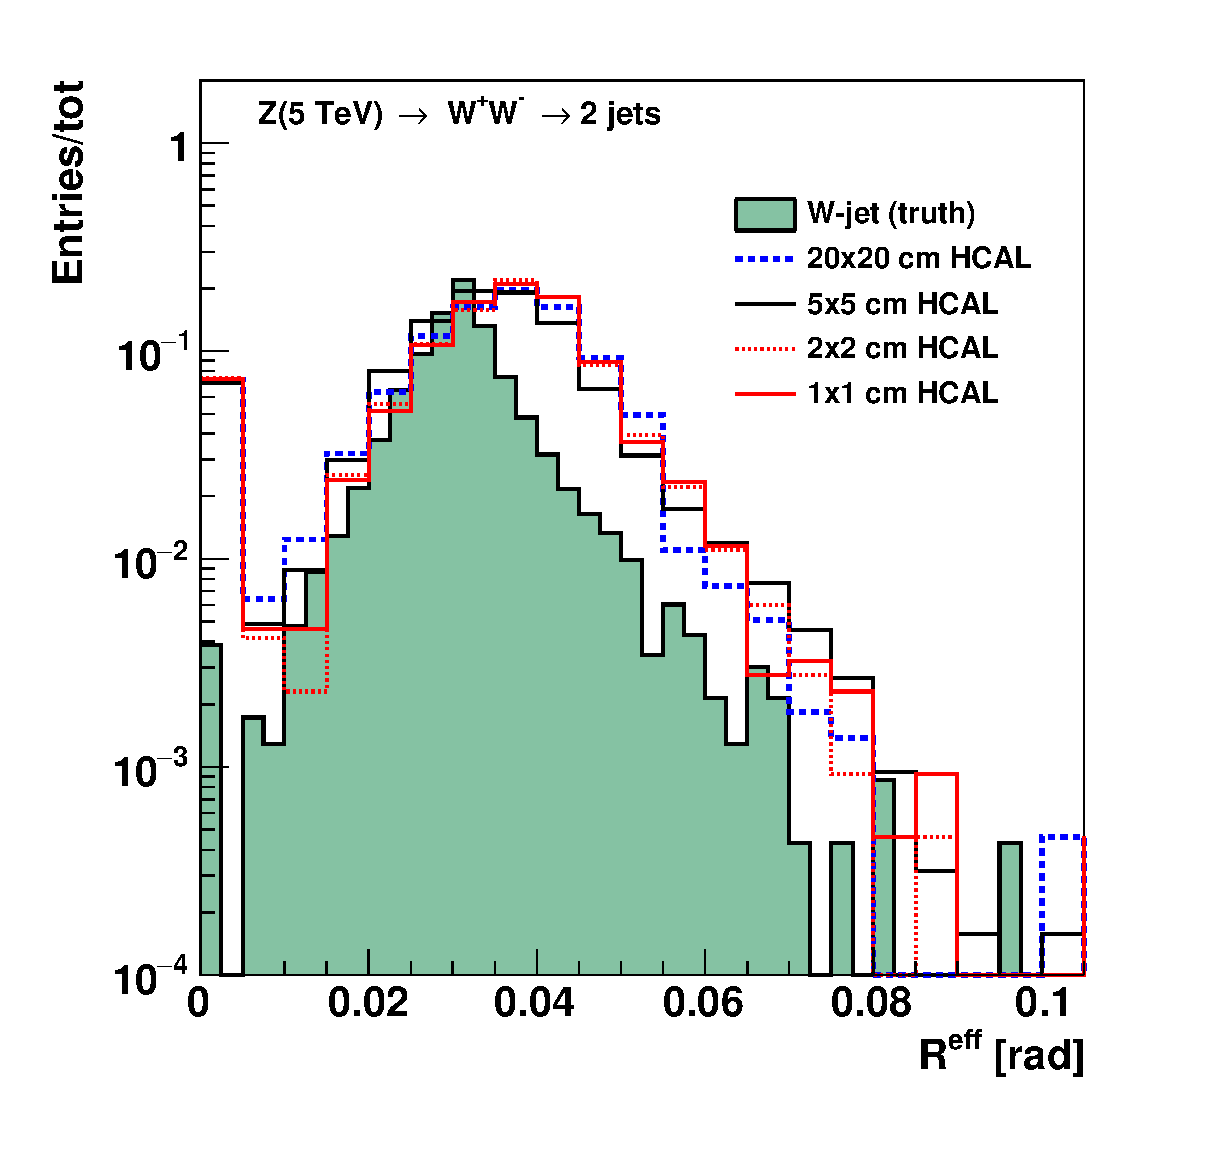
\includegraphics[width=0.43\textwidth]{figs/h5tev_clus_effR_ww1}\hfill
   }
   \subfigure[10 TeV] {
   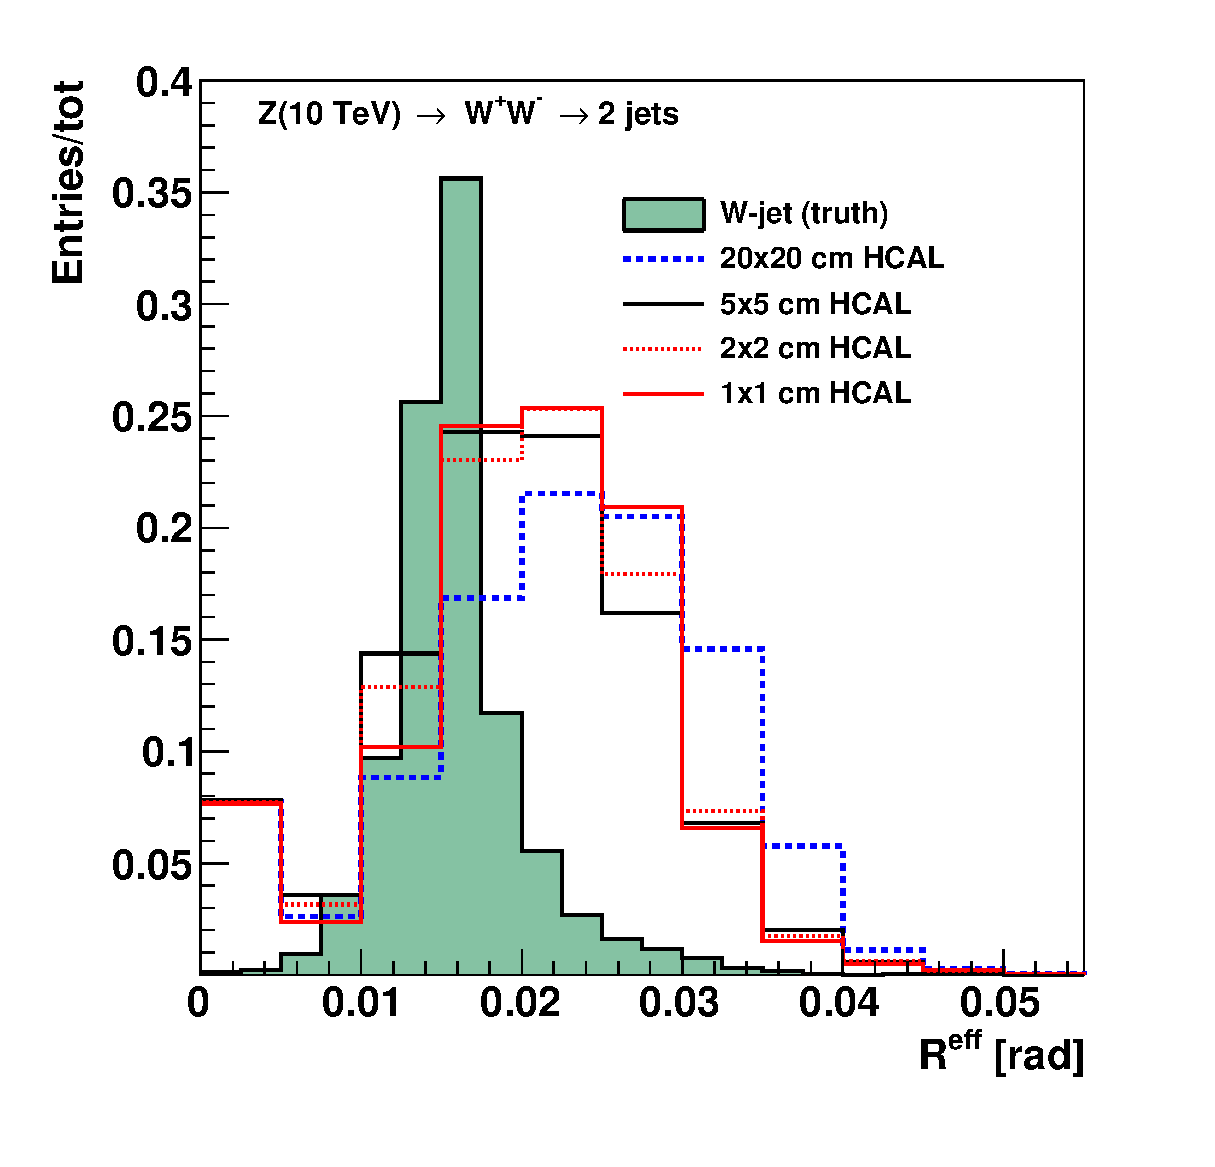
\includegraphics[width=0.43\textwidth]{figs/h10tev_clus_effR_ww1}
   }
   \subfigure[20 TeV] {
   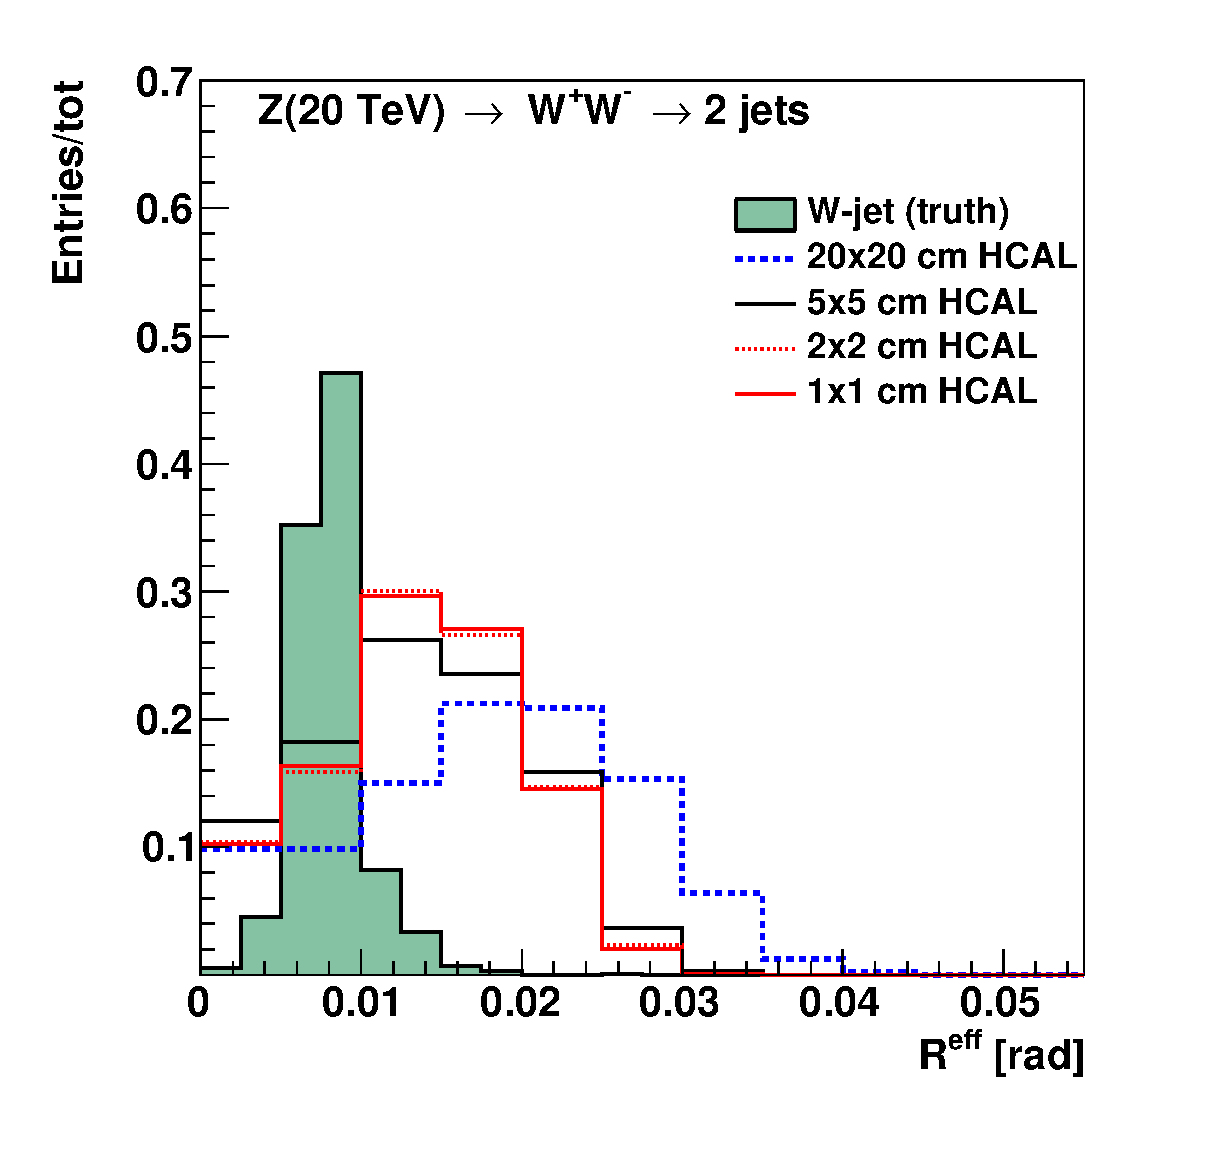
\includegraphics[width=0.43\textwidth]{figs/h20tev_clus_effR_ww1}
   }
   \subfigure[40 TeV] {
   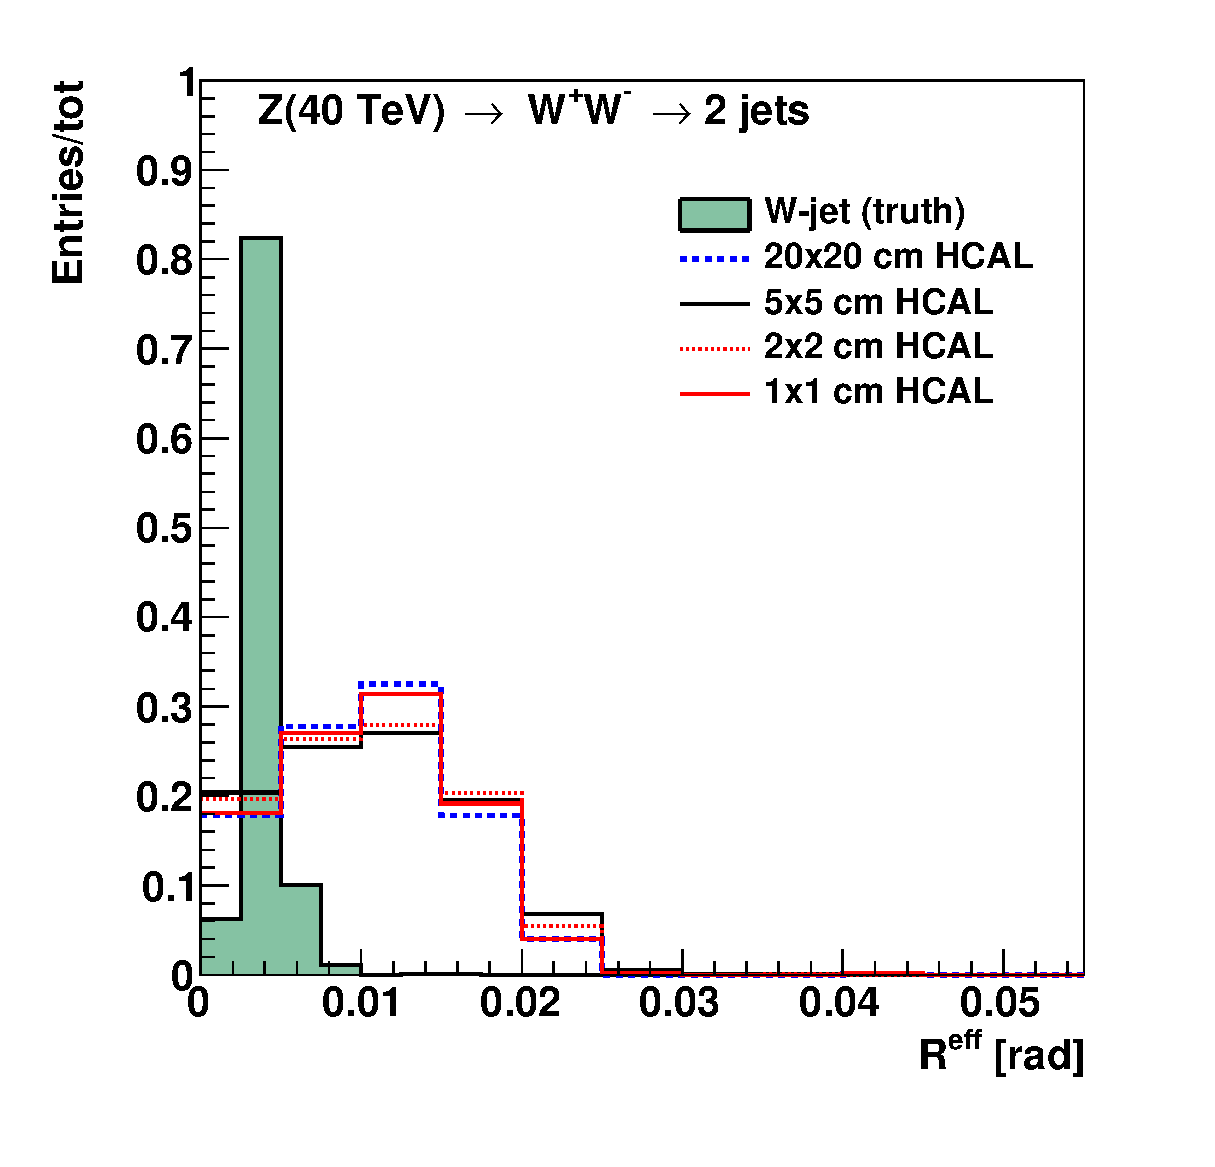
\includegraphics[width=0.43\textwidth]{figs/h40tev_clus_effR_ww1}
   }
\end{center}
\caption{Jet effective radius for different jet transverse moment and HCAL granularity.}
\label{fig:eff_rad}
\end{figure}


New we sill study jet splitting the effect of granularity on jet splitting scales.
A jet $k_T$ splitting scale \cite{Butterworth:2002tt} is defined as a distance measure
used to form jets by the $k_T$ recombination
algorithm \cite{Catani1993187,Ellis:1993tq}.
This has been studied by ATLAS~\cite{ATLAS:2012am}, and more recently in the context of 100 TeV physics \cite{Auerbach:2014xua}.
The distribution of the splitting scale $\sqrt{d_{12}}=\min(p_T^1,p_T^2) \times \delta R_{12}$ \cite{ATLAS:2012am} at the final stage of the $k_T$ clustering, where two subjets are merged into the final one,
is shown in Fig.~\ref{fig:d12}.

\begin{figure}
\begin{center}
   \subfigure[5 TeV] {
   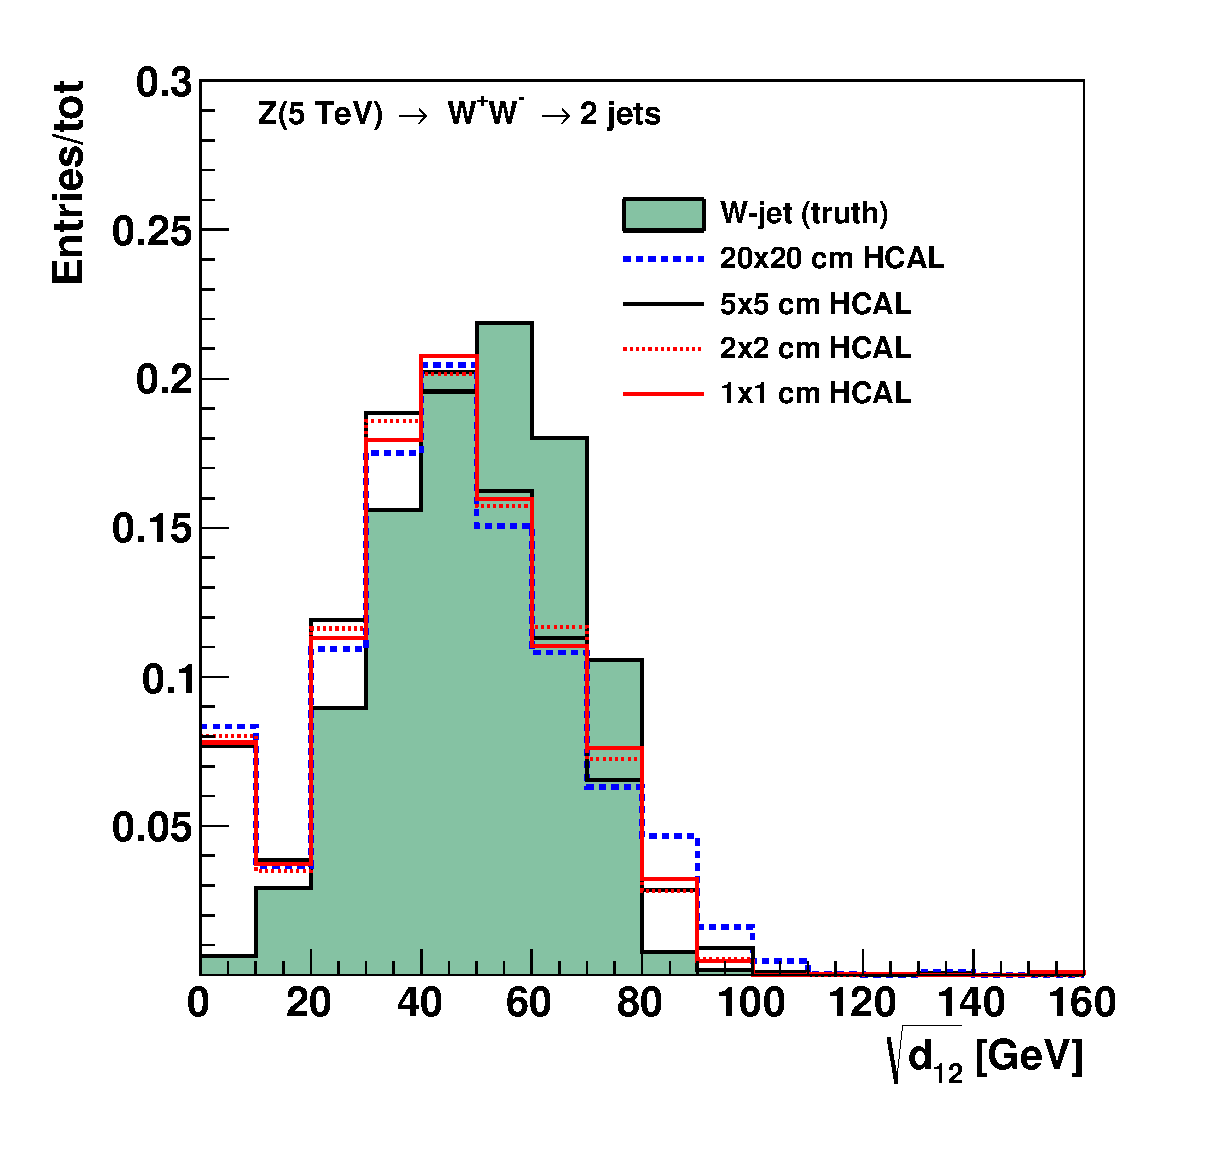
\includegraphics[width=0.43\textwidth]{figs/h5tev_clus_d12_ww1}\hfill
   }
   \subfigure[10 TeV] {
   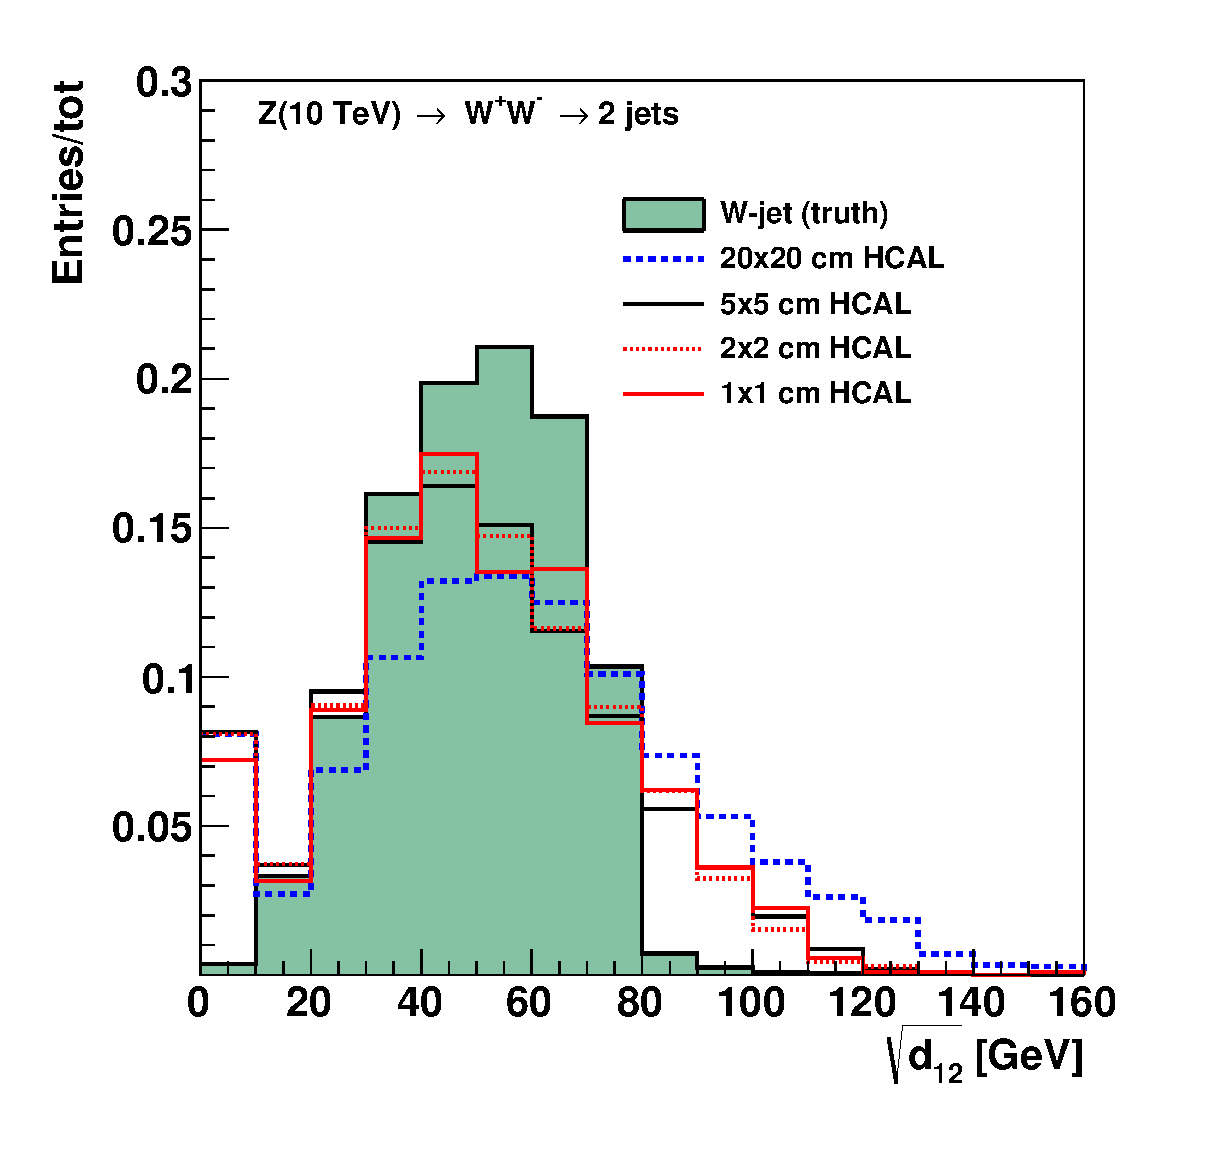
\includegraphics[width=0.43\textwidth]{figs/h10tev_clus_d12_ww1}
   }
   \subfigure[20 TeV] {
   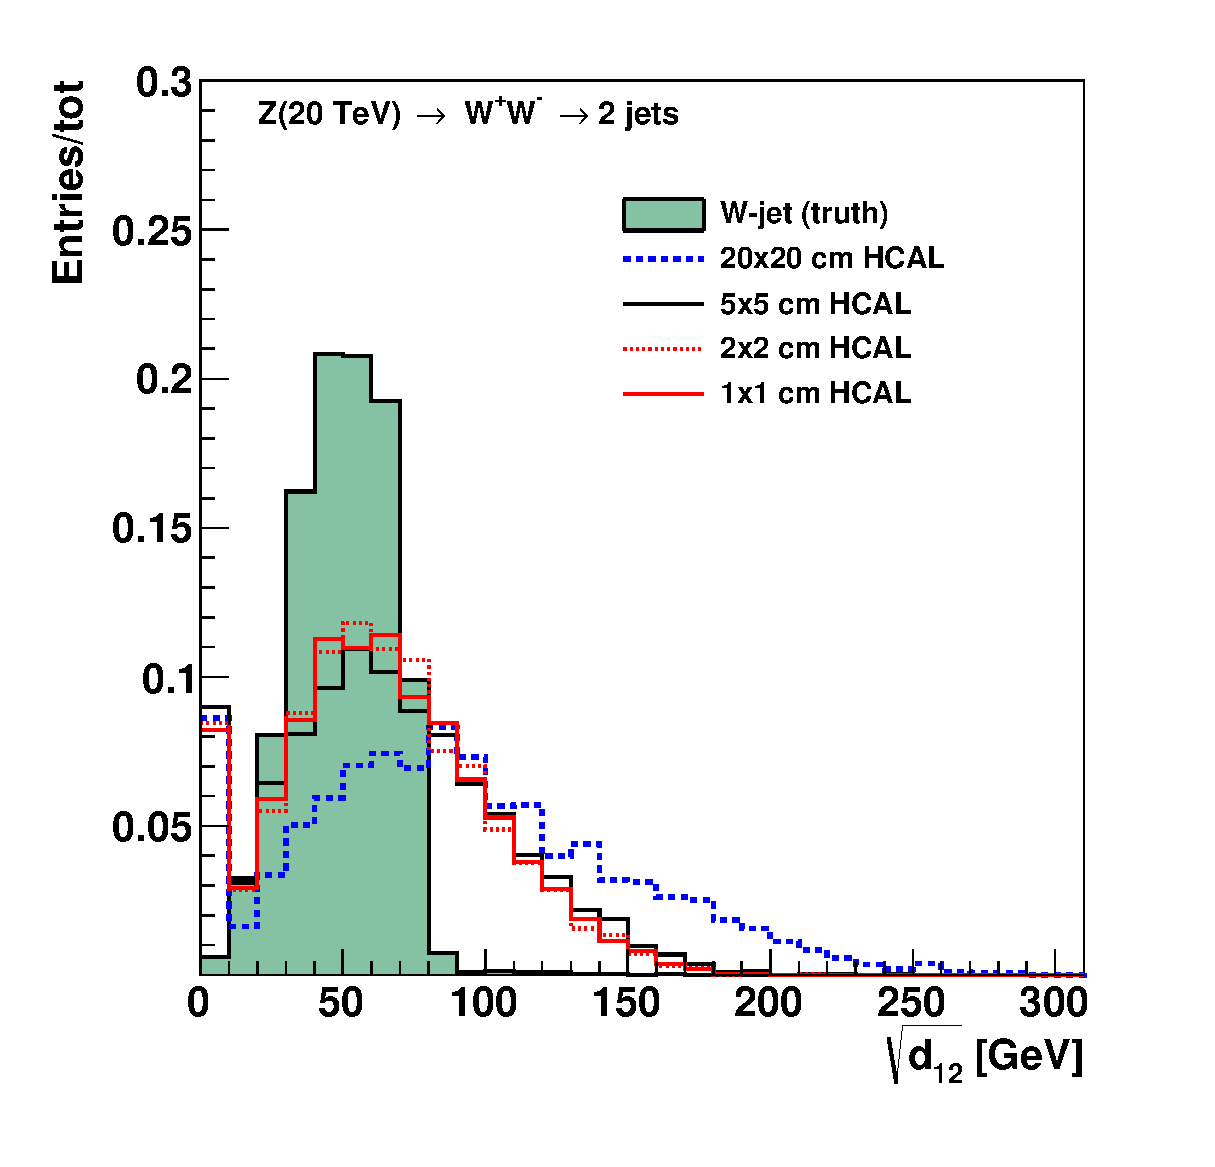
\includegraphics[width=0.43\textwidth]{figs/h20tev_clus_d12_ww1}
   }
   \subfigure[40 TeV] {
   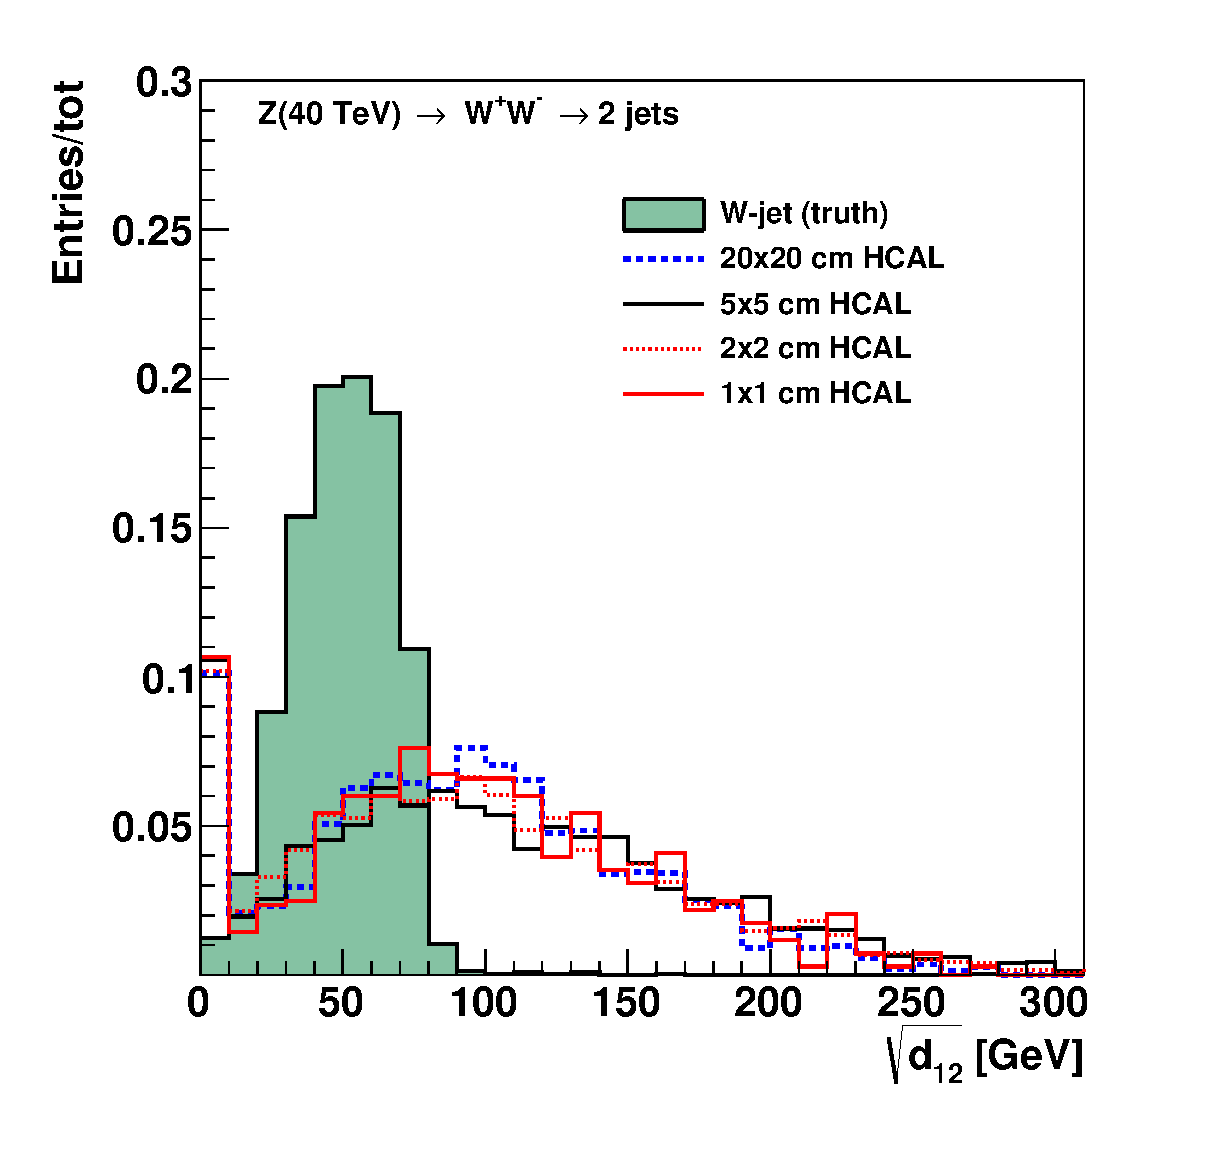
\includegraphics[width=0.43\textwidth]{figs/h40tev_clus_d12_ww1}
   }
\end{center}
\caption{Jet splitting scale for different jet transverse moment and HCAL granularity.}
\label{fig:d12}
\end{figure}






\section{Studies of signal and background separation using calorimeter clusters}
%%In the future detector, when the energy is increased, the boost jet is bigger, and it will be more difficult to distinguish the signal and the background. In this section, we want to study different variables and see their ability to separate the signal and the background in different detector sizes in the clustering of detector-level.\\
In this section, we study different jet substructure variables and compare their ability to separate the signal and the background for different detector sizes using calorimeter clusters.\\
%%Figure 3 to 5 show the ROC curves of three variables, $c2b1$ , $\tau_{21}$, and $\tau_{32}$. For each variable, there are three different sizes of the sub-detector HCAL compared at four special collision energies. For different sizes, the one with the highest background rejection rate, which is 1-background efficiency, at the same signal efficiency has the best separate ability.

Figures \textcolor{blue}{3}--\textcolor{blue}{5} show the ROC curves of three variables, $c_2^{(1)}$~\cite{Larkoski:2013eya} , $\tau_{21}$~\cite{Thaler:2010tr}, and $\tau_{32}$~\cite{Thaler:2010tr}, respectively. Three different cell sizes of the HCAL are compared for four collision energies. For different cell sizes with the same signal efficiency, the one with the highest background rejection rate, namely (1-background efficiency), has the highest separate power.\\

In Figure \textcolor{blue}{3} for the variable $c_2^{(1)}$ , the ROC curves of the three detector cell sizes are close to each other for each collision energy. Therefore, this variable is not sensitive to the detector cell size.\\

For the $\tau_{21}$ variable in Figure \textcolor{blue}{4}, at 5 TeV, the smallest detector size (1$\times$1 cm) can separate the background from the signal well. However, this is not the usual case as the ROC curves nearly merge together at higher collision energy. In addition, the detector with the bigger size tends to have higher separation power than the smaller detector size in 20 and 40 TeV collision energy.\\

Figure \textcolor{blue}{5} shows the variable $\tau_{32}$, where the smallest detector size has the best separation power for all collision energies.\\

In conclusion, in all the cases of energy and detector size, the variable $c_2^{(1)}$ has the best separation power compared to the other two variables. In addition, the variable $\tau_{32}$ follows the expectation that smaller detector size has better separation power.\\

\label{sec:efficiency}


\begin{figure}
\begin{center}
   \subfigure[5 TeV] {
   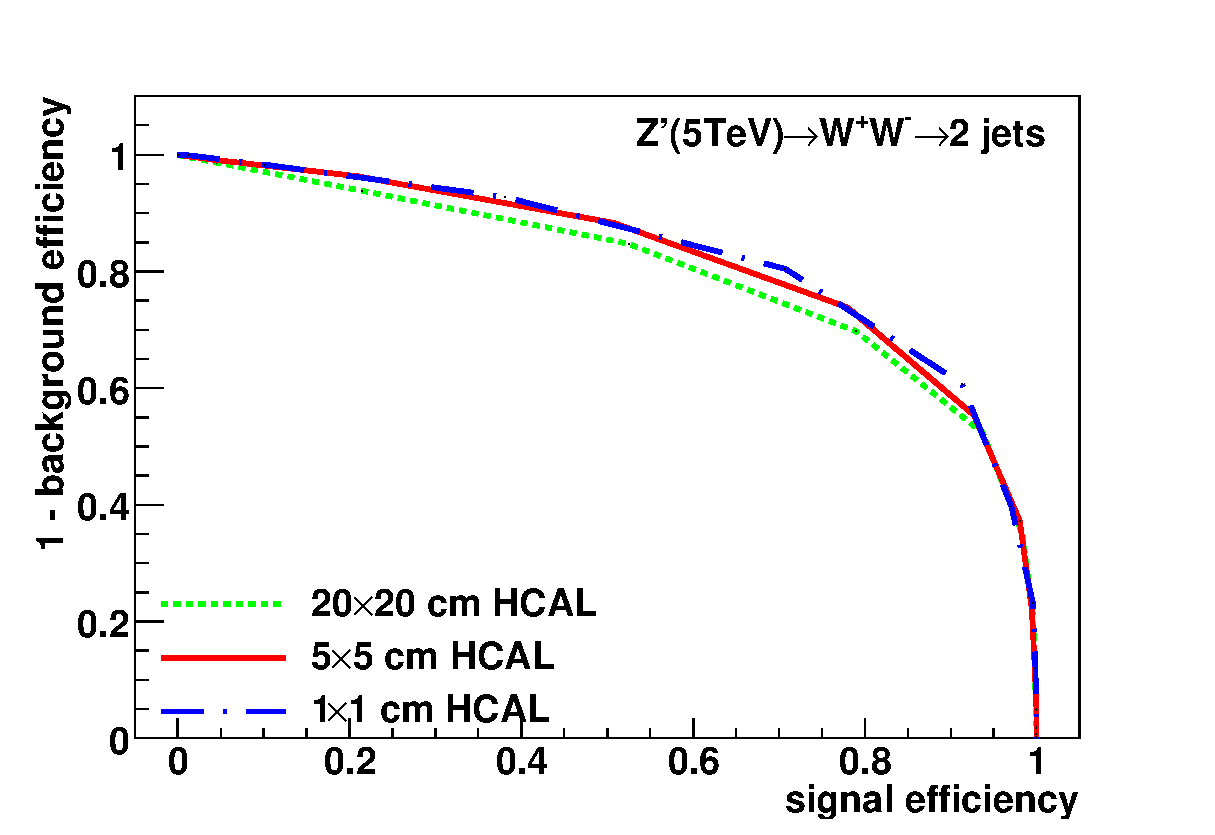
\includegraphics[width=0.43\textwidth]{figs/cluster_c2b1_5_tev_eff.eps}\hfill
   }
   \subfigure[10 TeV] {
   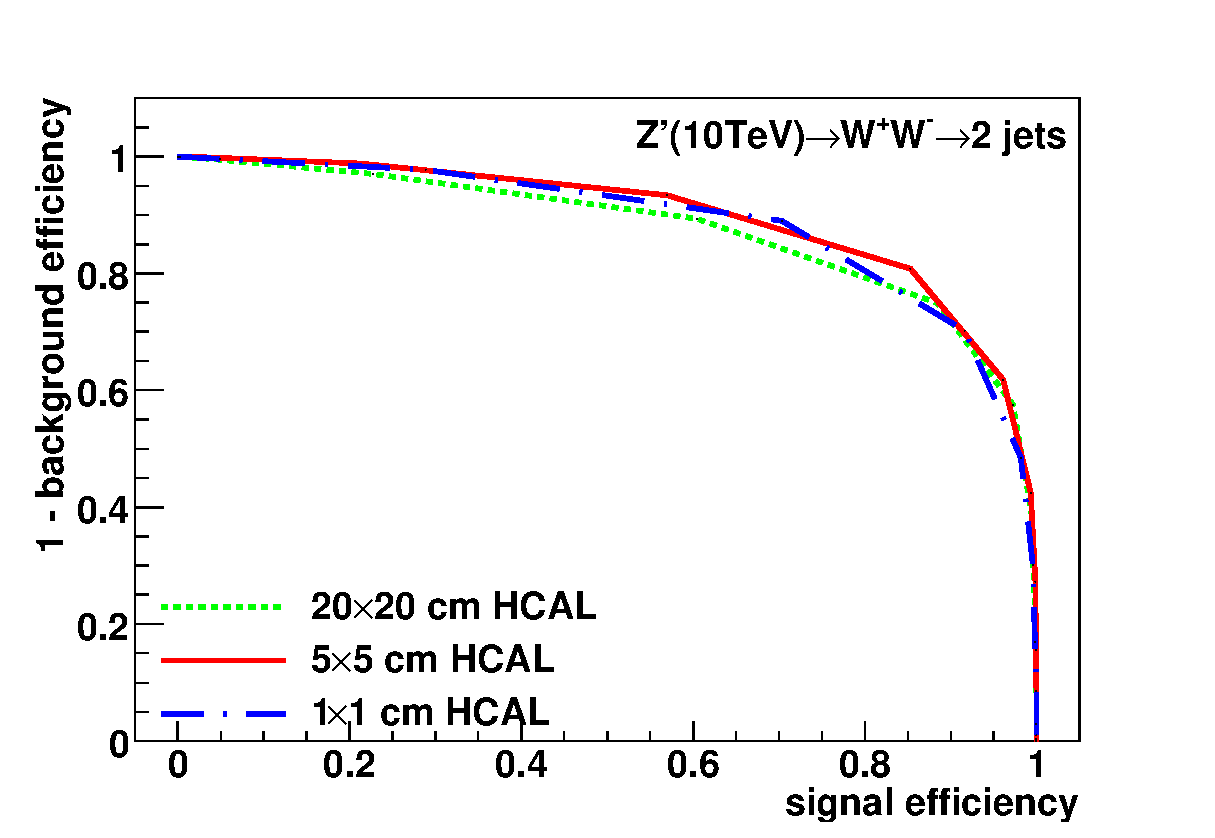
\includegraphics[width=0.43\textwidth]{figs/cluster_c2b1_10_tev_eff.eps}
   }
   \subfigure[20 TeV] {
   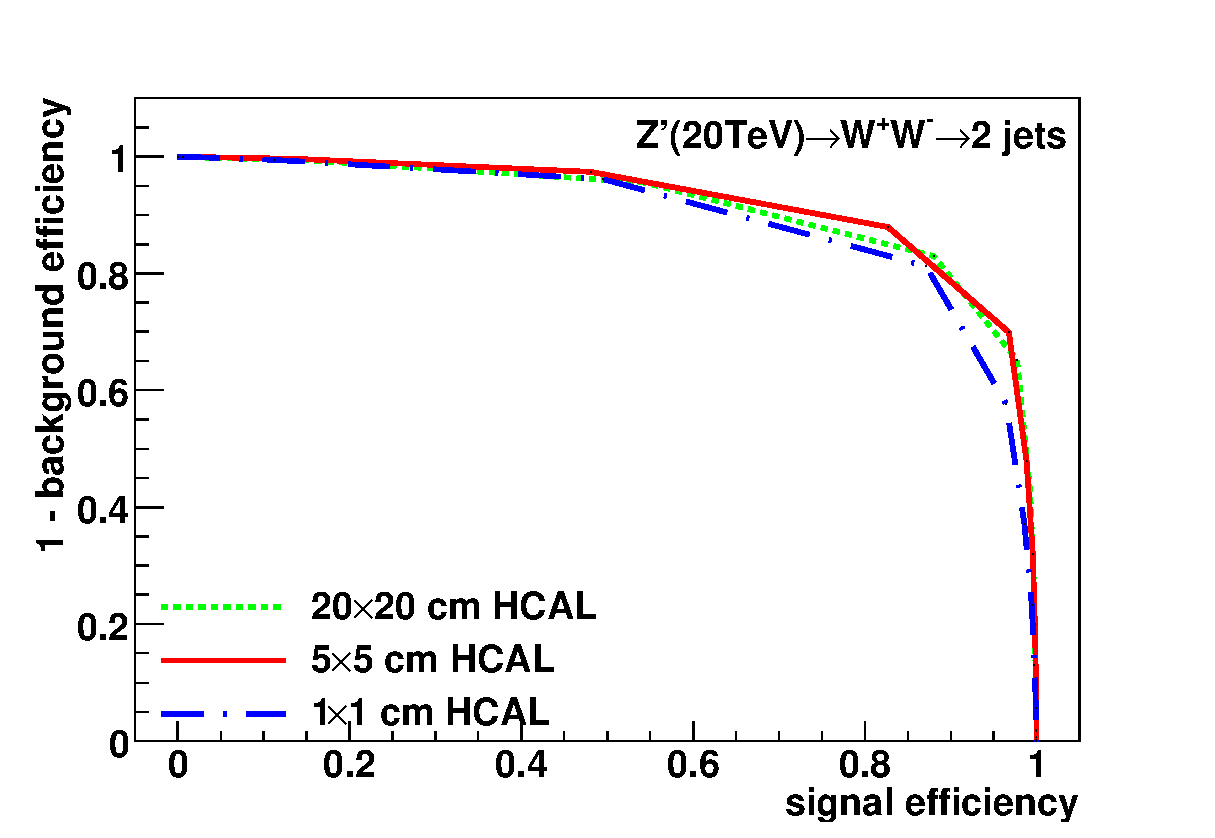
\includegraphics[width=0.43\textwidth]{figs/cluster_c2b1_20_tev_eff.eps}
   }
   \subfigure[40 TeV] {
   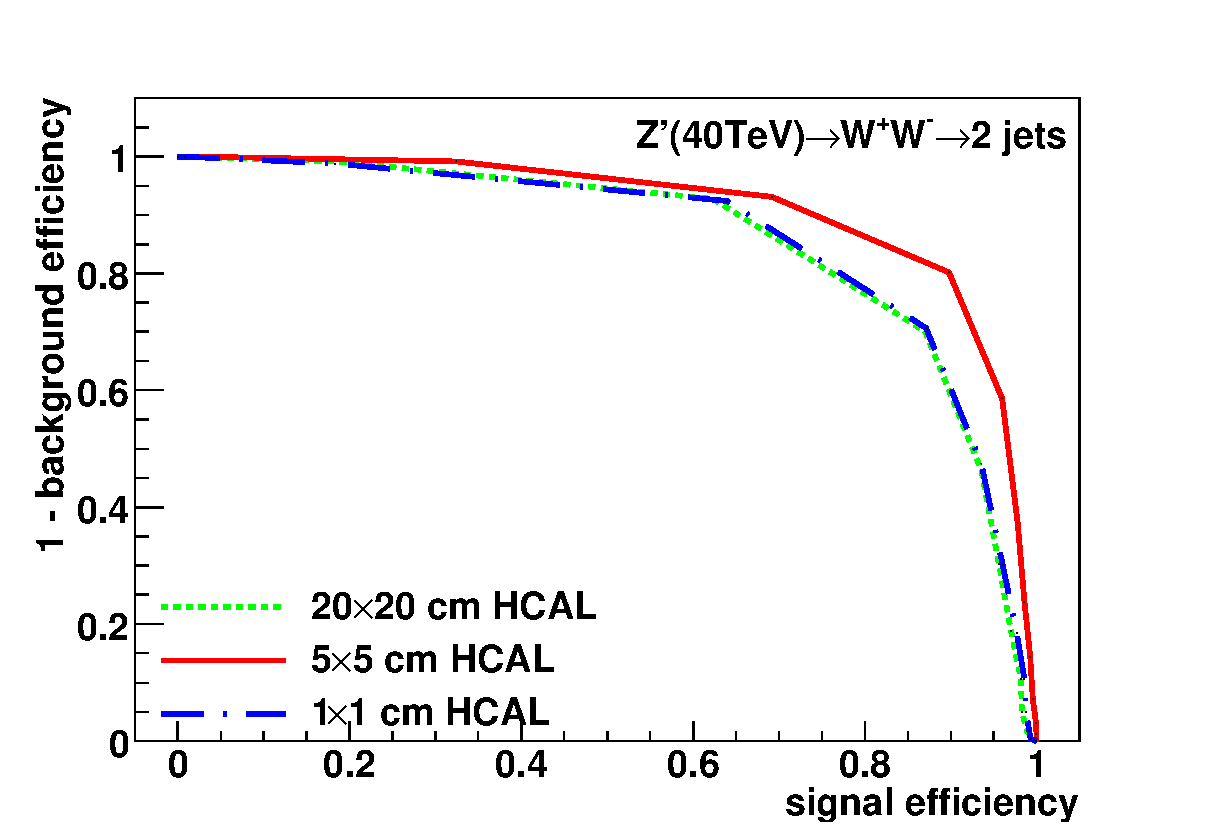
\includegraphics[width=0.43\textwidth]{figs/cluster_c2b1_40_tev_eff.eps}
   }
\end{center}
\caption{Signal efficiency versus background rejection rate using $c_2^{(1)}$.The energies of collision at (a)5, (b)10, (c)20, (d)40TeV are shown here. In each picture, the three ROC curves correspond to different detector sizes.}
\label{fig:cluster_c2b1}
\end{figure}


\begin{figure}
\begin{center}
   \subfigure[5 TeV] {
   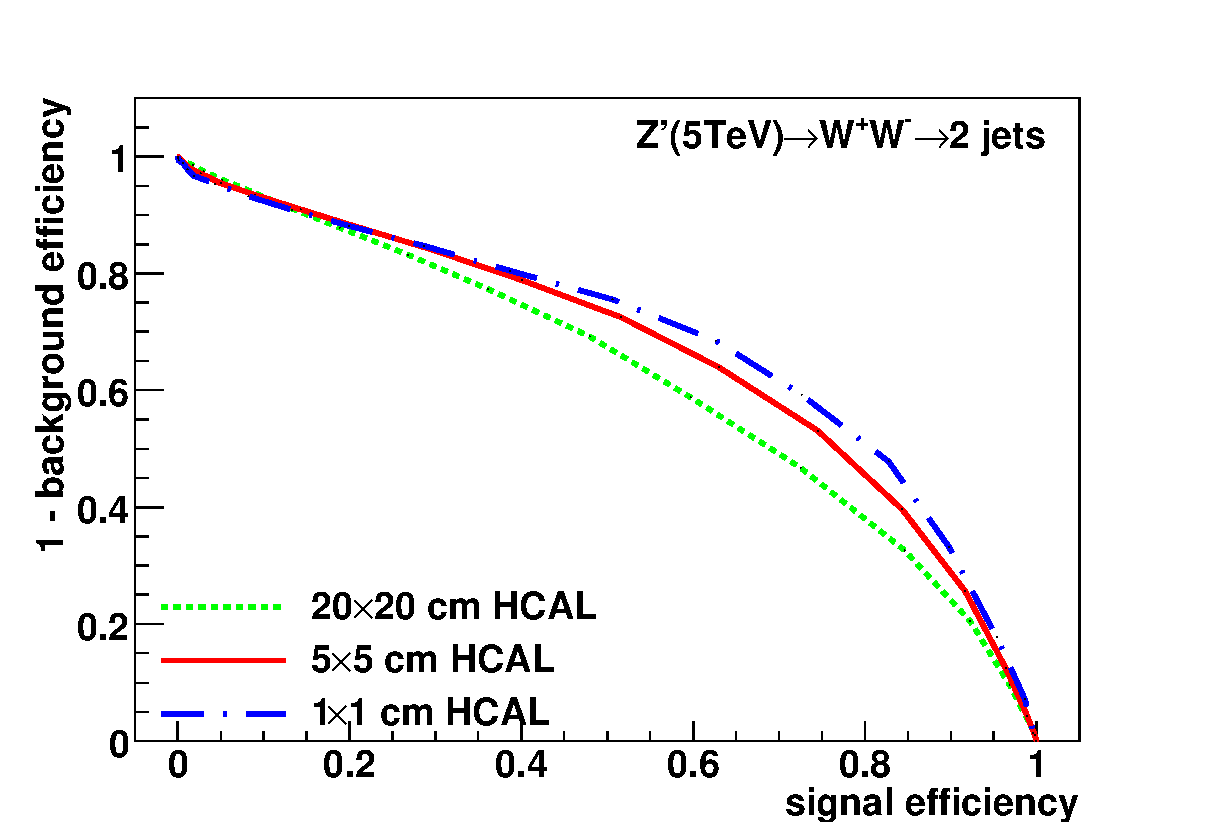
\includegraphics[width=0.43\textwidth]{figs/cluster_tau21_5_tev_eff.eps}\hfill
   }
   \subfigure[10 TeV] {
   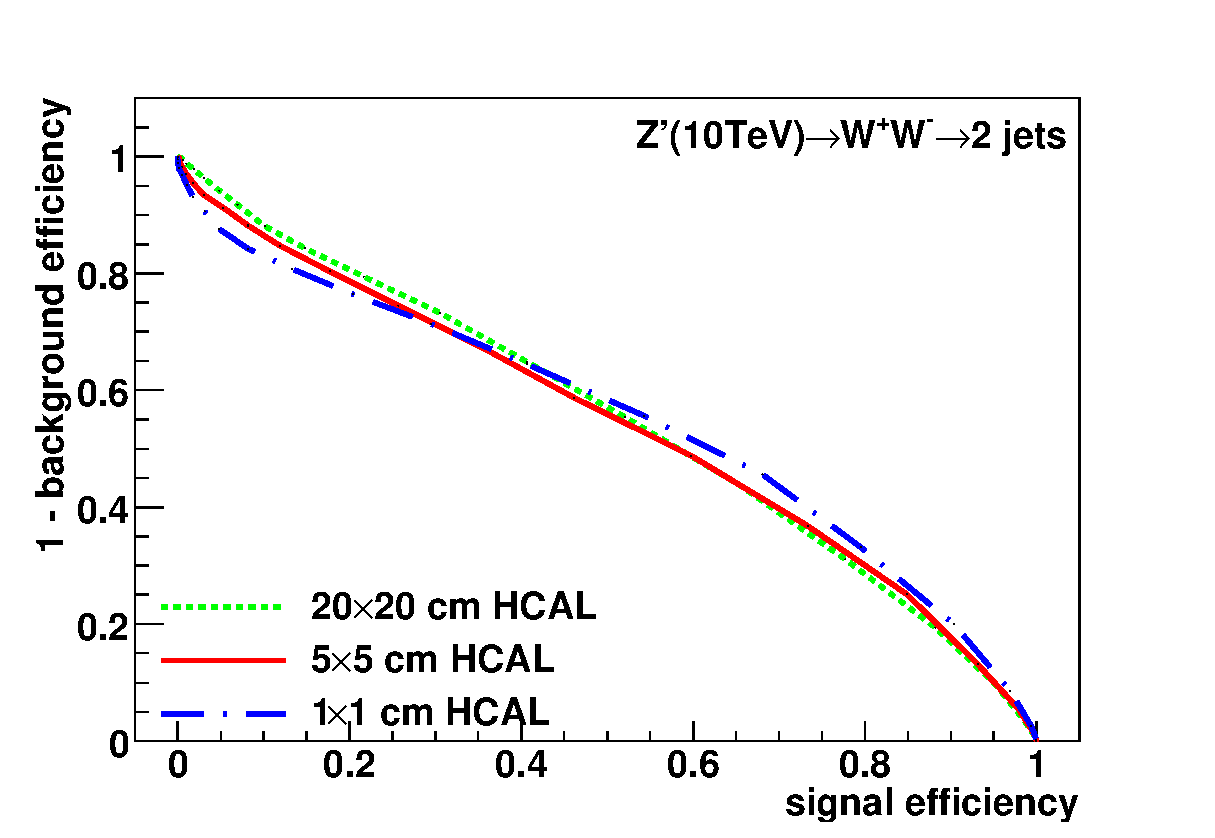
\includegraphics[width=0.43\textwidth]{figs/cluster_tau21_10_tev_eff.eps}
   }
   \subfigure[20 TeV] {
   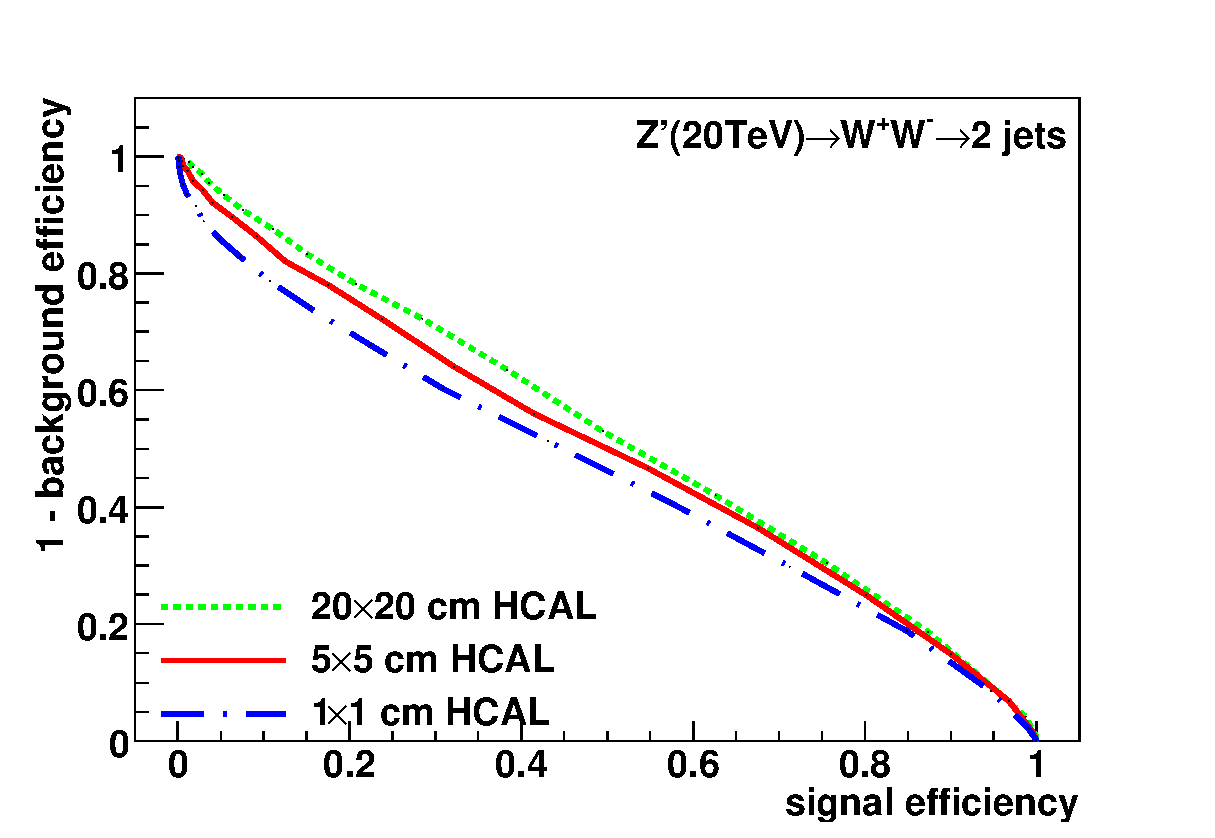
\includegraphics[width=0.43\textwidth]{figs/cluster_tau21_20_tev_eff.eps}
   }
   \subfigure[40 TeV] {
   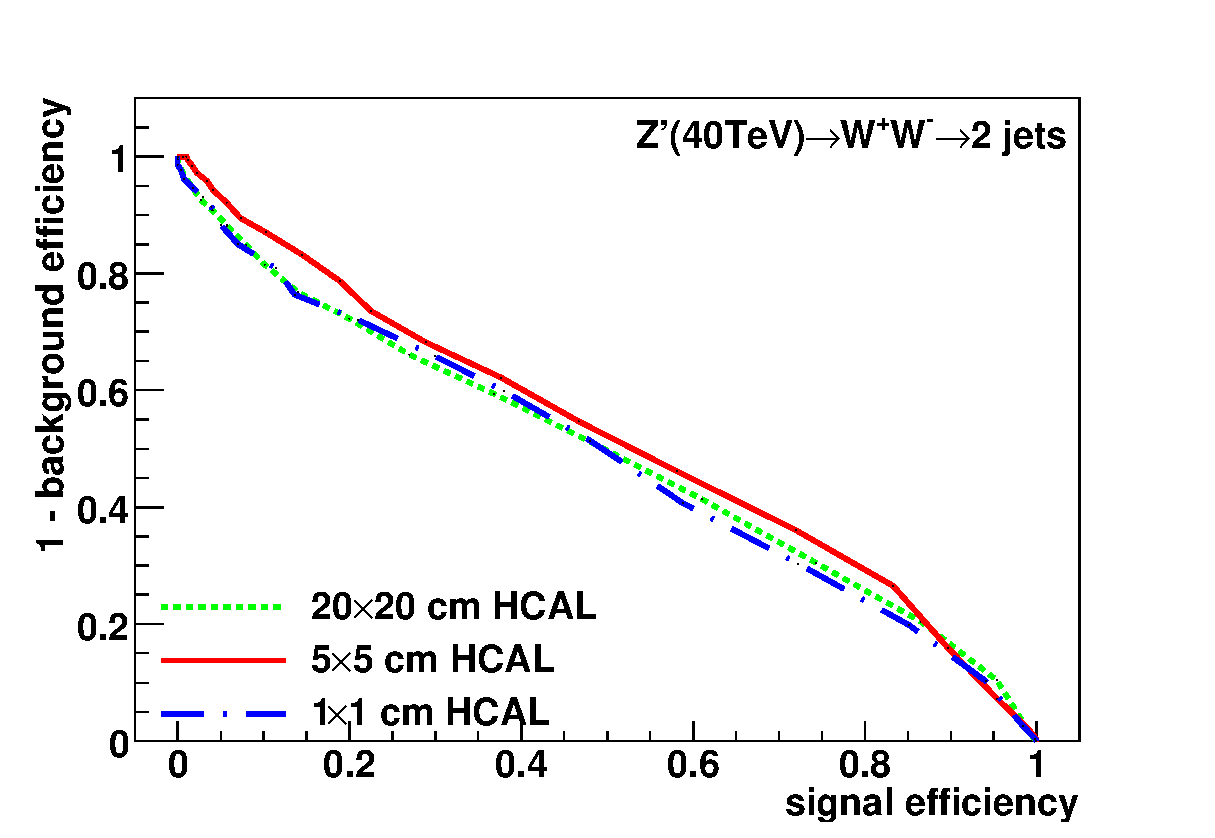
\includegraphics[width=0.43\textwidth]{figs/cluster_tau21_40_tev_eff.eps}
   }
\end{center}
\caption{Signal efficiency versus background rejection rate using $\tau_{21}$.The energies of collision at (a)5, (b)10, (c)20, (d)40TeV are shown here. In each picture, the three ROC curves correspond to different detector sizes.}
\label{fig:cluster_tau21}
\end{figure}


\begin{figure}
\begin{center}
   \subfigure[5 TeV] {
   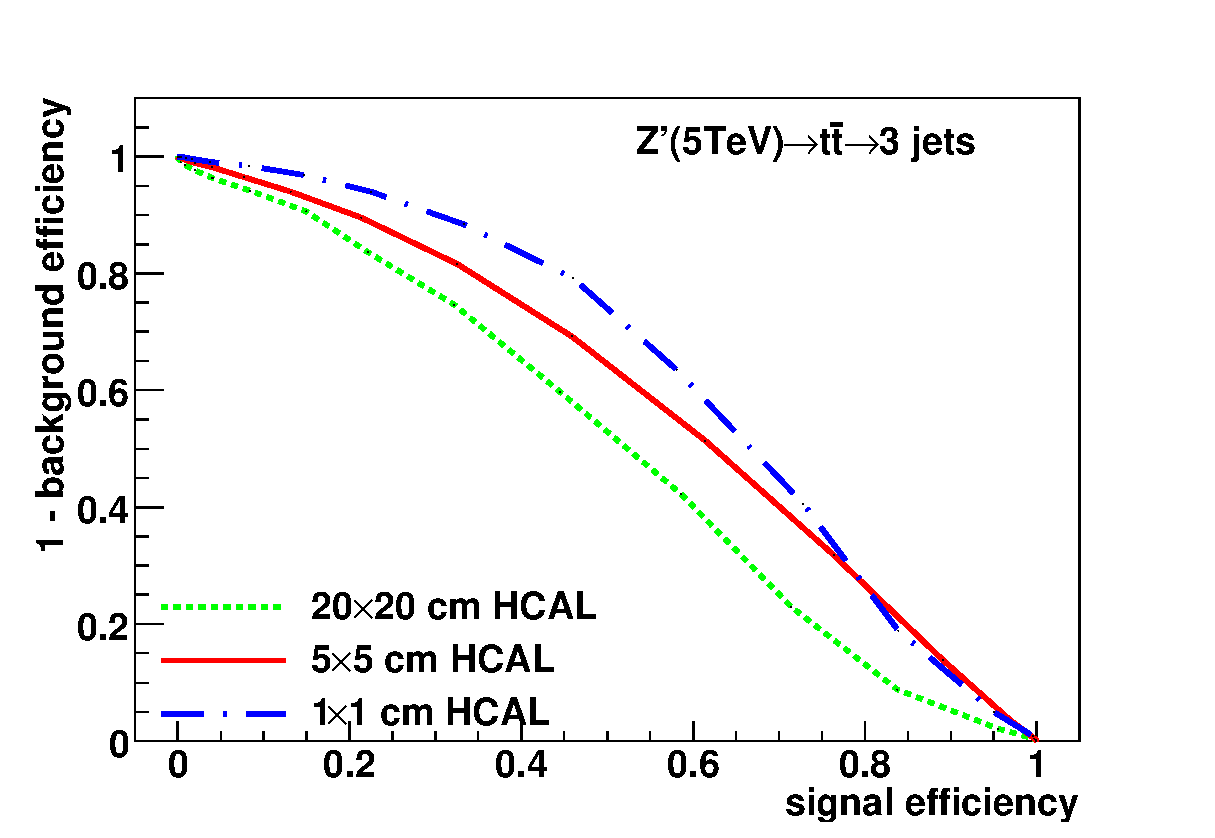
\includegraphics[width=0.43\textwidth]{figs/cluster_tau32_5_tev_eff.eps}\hfill
   }
   \subfigure[10 TeV] {
   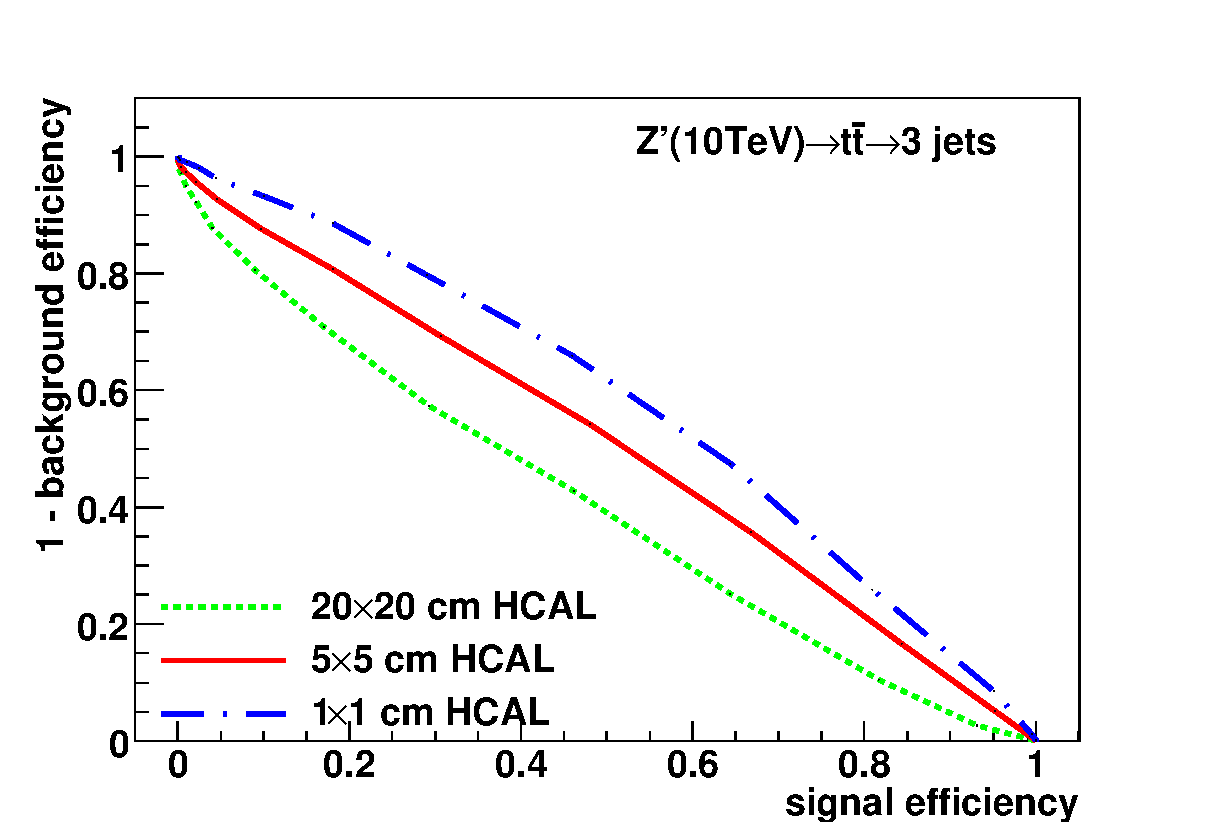
\includegraphics[width=0.43\textwidth]{figs/cluster_tau32_10_tev_eff.eps}
   }
   \subfigure[20 TeV] {
   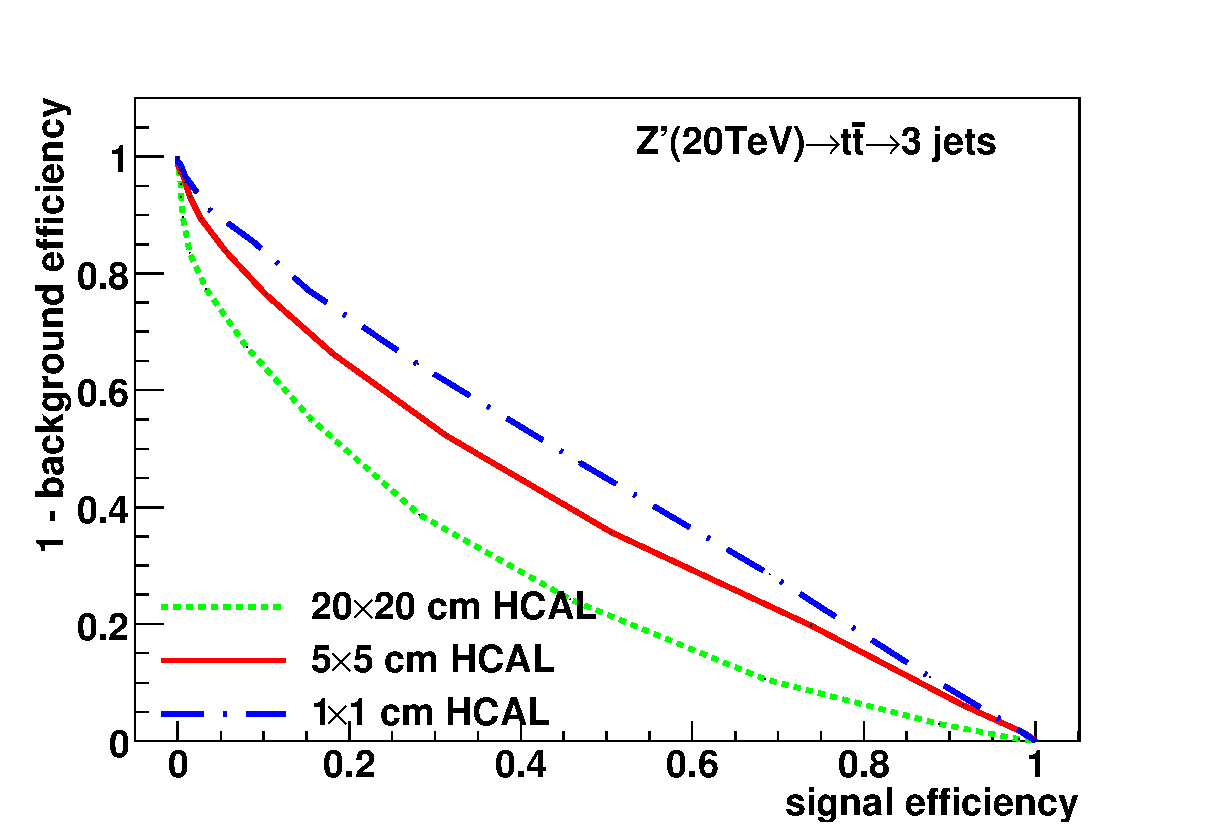
\includegraphics[width=0.43\textwidth]{figs/cluster_tau32_20_tev_eff.eps}
   }
   \subfigure[40 TeV] {
   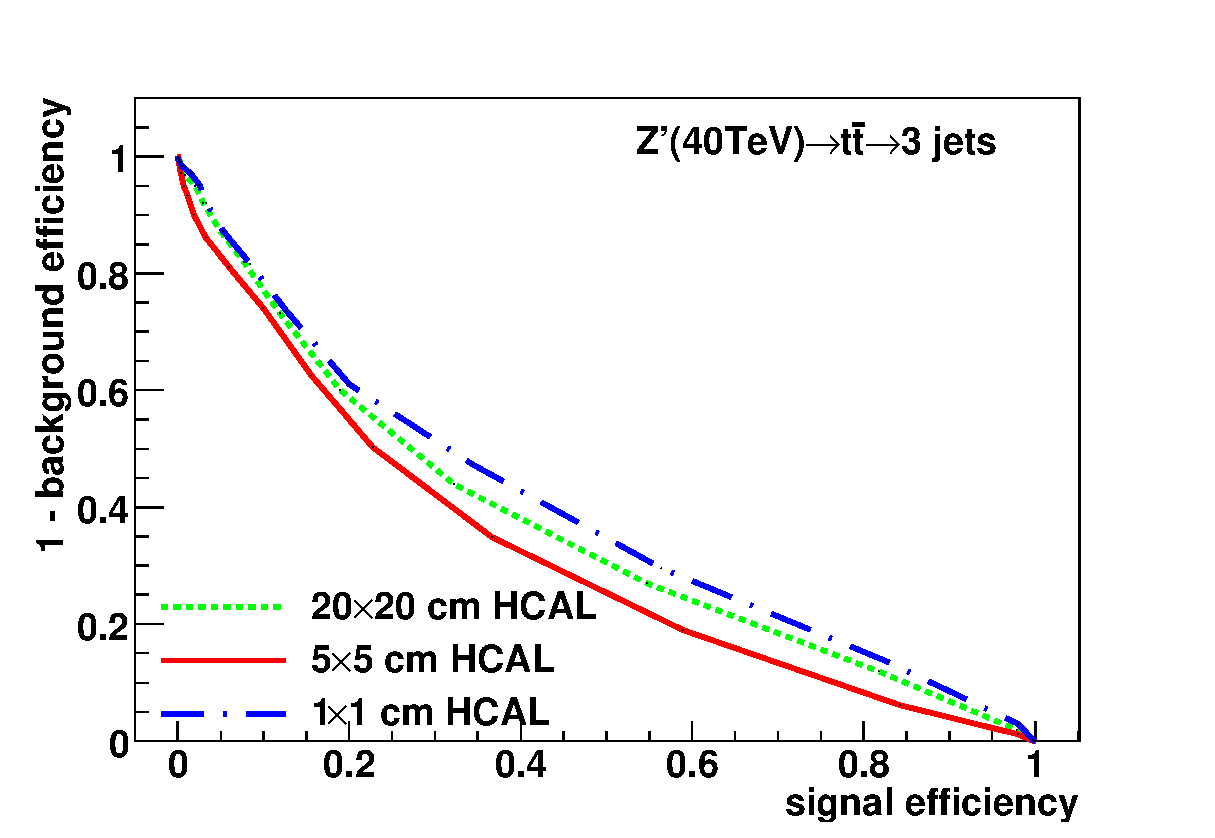
\includegraphics[width=0.43\textwidth]{figs/cluster_tau32_40_tev_eff.eps}
   }
\end{center}
\caption{Signal efficiency versus background rejection rate using $\tau_{32}$.The energies of collision at (a)5, (b)10, (c)20, (d)40TeV are shown here. In each picture, the three ROC curves correspond to different detector sizes.}
\label{fig:cluster_tau32}
\end{figure}



\section{Studies of signal and background separation using Mann-Whitney U test}
%In this section, we study different jet substructure variables and compare their ability to separate the signal and the background for different detector sizes using Mann-Whitney U test.\\

%In the Mann Whitney U test by definition, if U value is closed to 0.5, it means two distributions have similar compositions, and we can't distinguish them very well. On the other hand, if U value of two distributions are closed to 0, it means both distributions' compositions are much different from each other. For another point of view, if U value is closed to 0.5, separation power of certain variable is bad, instead, if U value is closed to 0, separation power is great.\\

%Figure 6 shows the representative samples of the distributions about the U value for $\tau_{21}$,$\tau_{32}$ in different detector sizes. In $\tau_{21}$, separation power is improved when detector size is smaller, but in $\tau_{32}$, the smallest detector sizes isn't the best one to separate signal and background.\\

%In Figure 7, it shows the summary plots about the clustering in Mann Whitney U test in three different variables. In $\tau_{21}$, 5TeV has better separation power when detector sizes are getting smaller, but when energy higher than that, there is no improvement in smaller detector. In $\tau_{32}$, the case is similar to  $\tau_{21}$. Even worse, at some collision energies, bigger detector sizes have better separation power than smaller detector sizes. In $c_2^{(1)}$, all separation power aren't improved by detector sizes.  In summary, $c_2^{(1)}$ is the best parameter, because all values are smaller than other parameters compare with the same energy collision, and its separation power don't have the significant improvement in higher energy collision.\\

%In Figure 8 , it shows the summary plots about the rawhit cut at 0.5GeV in Mann Whitney U test in three different variables. In $\tau_{21}$, 5TeV and 10TeV have better separation power in smaller separation power, but when energy higher than that, it won't improve.  In $\tau_{32}$, all separation power aren't improved by detector sizes. In $c_2^{(1)}$, we can see in 5,10,20TeV, separation power will be improved slightly, but at 40TeV, it won't improve. In summary, $c_2^{(1)}$ has the highest power separation at highest collision energy.\\

In this section, we studied different jet substructure variables and compared their ability to separate the signal and background for different detector sizes using the Mann-Whitney U test.\\

By the definition of the Mann-Whitney U test, if the value of U is close to 0.5, it means that the signal and background distribution have almost similar compositions. This also means that the separation power of the variable is bad. On the other hand, if the U value is close to 0, it means that the distribution of the signal and the background are much different from each other and the separation power of the variable is great.\\

Figure 6 shows the representative sample of the distributions for $\tau_{21}$,$\tau_{32}$, in different detector sizes with their corresponding U value. In $\tau_{21}$, the separation power is better when the detector size is smaller. However, the separation power of tau32 does not improve when the detector size gets smaller.\\

Figure 7 shows the summary plots of the clustering in Mann-Whitney U test for the three different variables.  In $\tau_{21}$, 5 TeV has the better separation power when the detector size is smaller. However, there is not much improvement in higher energy collisions. In $\tau_{32}$, 5 TeV has also better separation power on smaller detector size but higher energy collisions seem to have better separation power when the detector size is bigger. The $c_2^{(1)}$ does not seem to have any significant improvement in its separation power as the detector size gets smaller for all energy collision. Nevertheless, the U values of the $c_2^{(1)}$ are better than the$\tau_{21}$ and $\tau_{32}$. In conclusion, the $c_2^{(1)}$ variable is the best parameter as its separation power is better than the other variable and does not have a significant improvement in higher energy collision.\\

Figure 8 shows the summary plots of the rawhit cut at 0.5 GeV in Mann Whitney U test for the three different variables. In $\tau_{21}$, 5 and 10 TeV have better separation power on smaller detector sizes. However, there is no significant improvement in the separation power of higher energy collisions. The $\tau_{32}$ does not have any significant improvement in its separation power as the detector size gets smaller for all energy collision. Lastly, there is a slight improvement in separation power for 5, 10, and 20 TeV energy collision in $c_2^{(1)}$. At 40 TeV, no significant improvement is observed. In conclusion, the $c_2^{(1)}$ variable is the best parameter as it has the best separation power at 40 TeV energy collision than the other variables.\\

\label{sec:Mann Whitney U test}


\begin{figure}
\begin{center}
   \subfigure[20$\times$20(cm$\times$cm)] {
   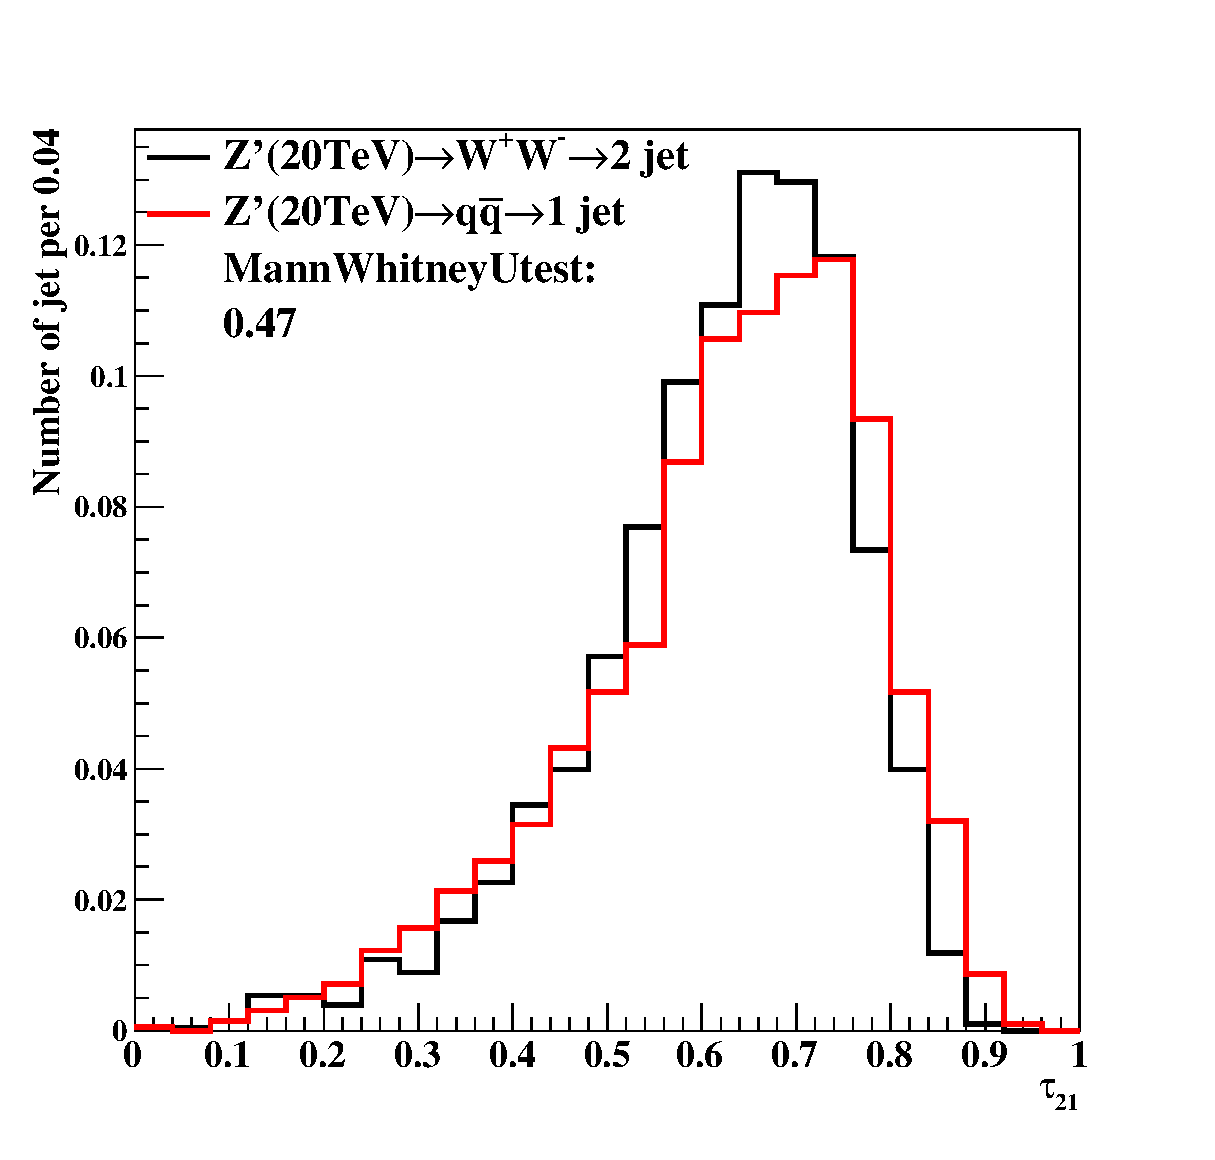
\includegraphics[width=0.43\textwidth]{figs/r010_tau21b1_20tev_04_U.eps}\hfill
   }
   \subfigure[20$\times$20(cm$\times$cm)] {
   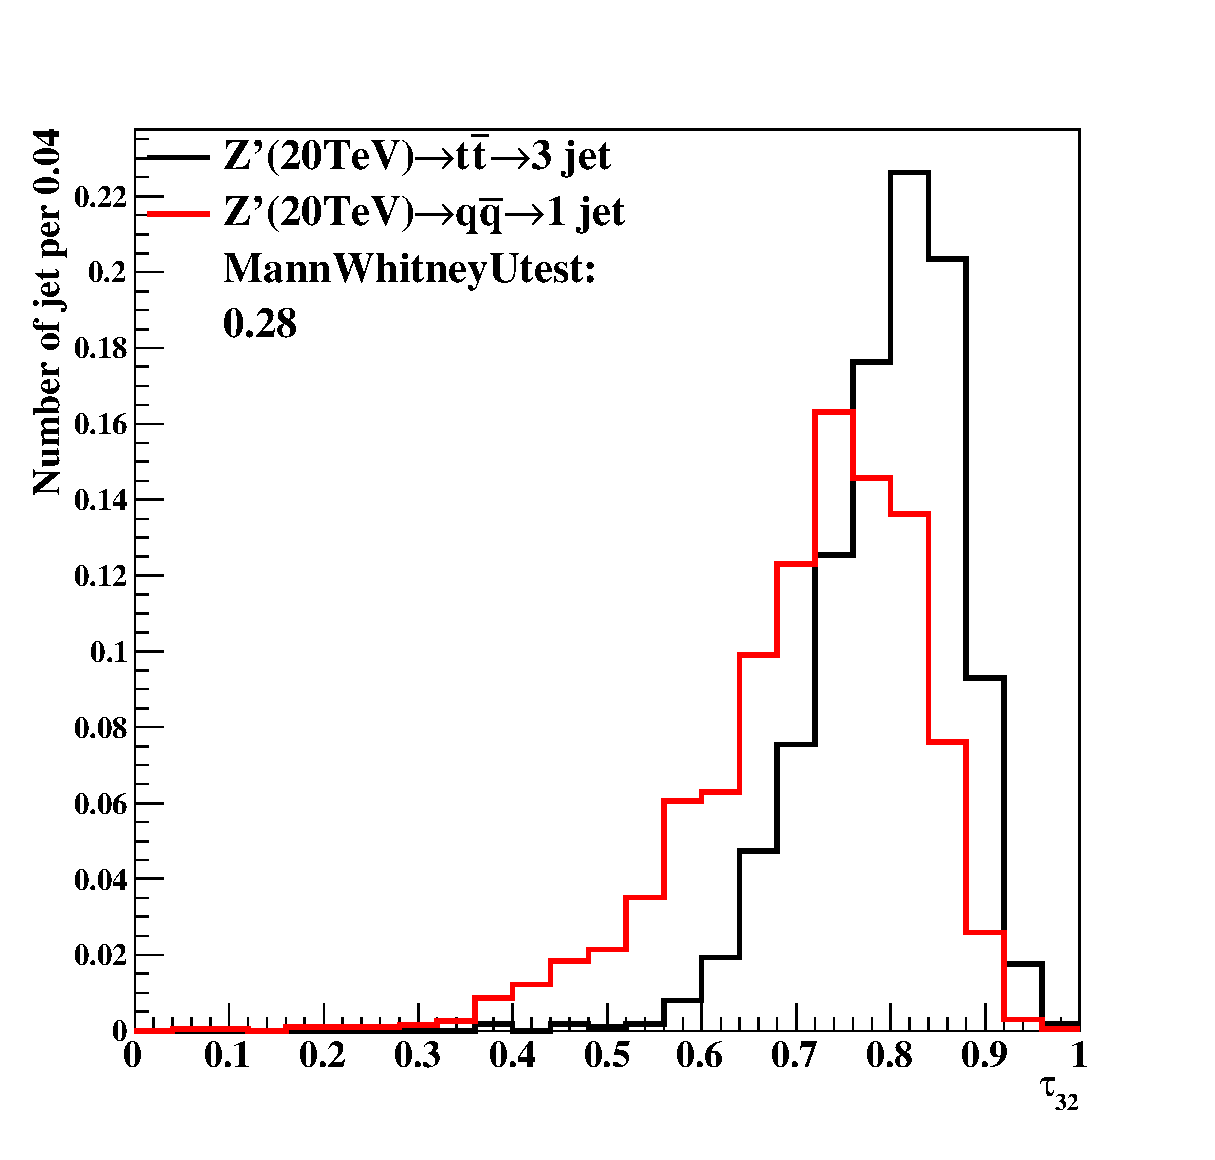
\includegraphics[width=0.43\textwidth]{figs/r010_tau32b1_20tev_04_U.eps}
   }
   \subfigure[5$\times$5(cm$\times$cm)] {
   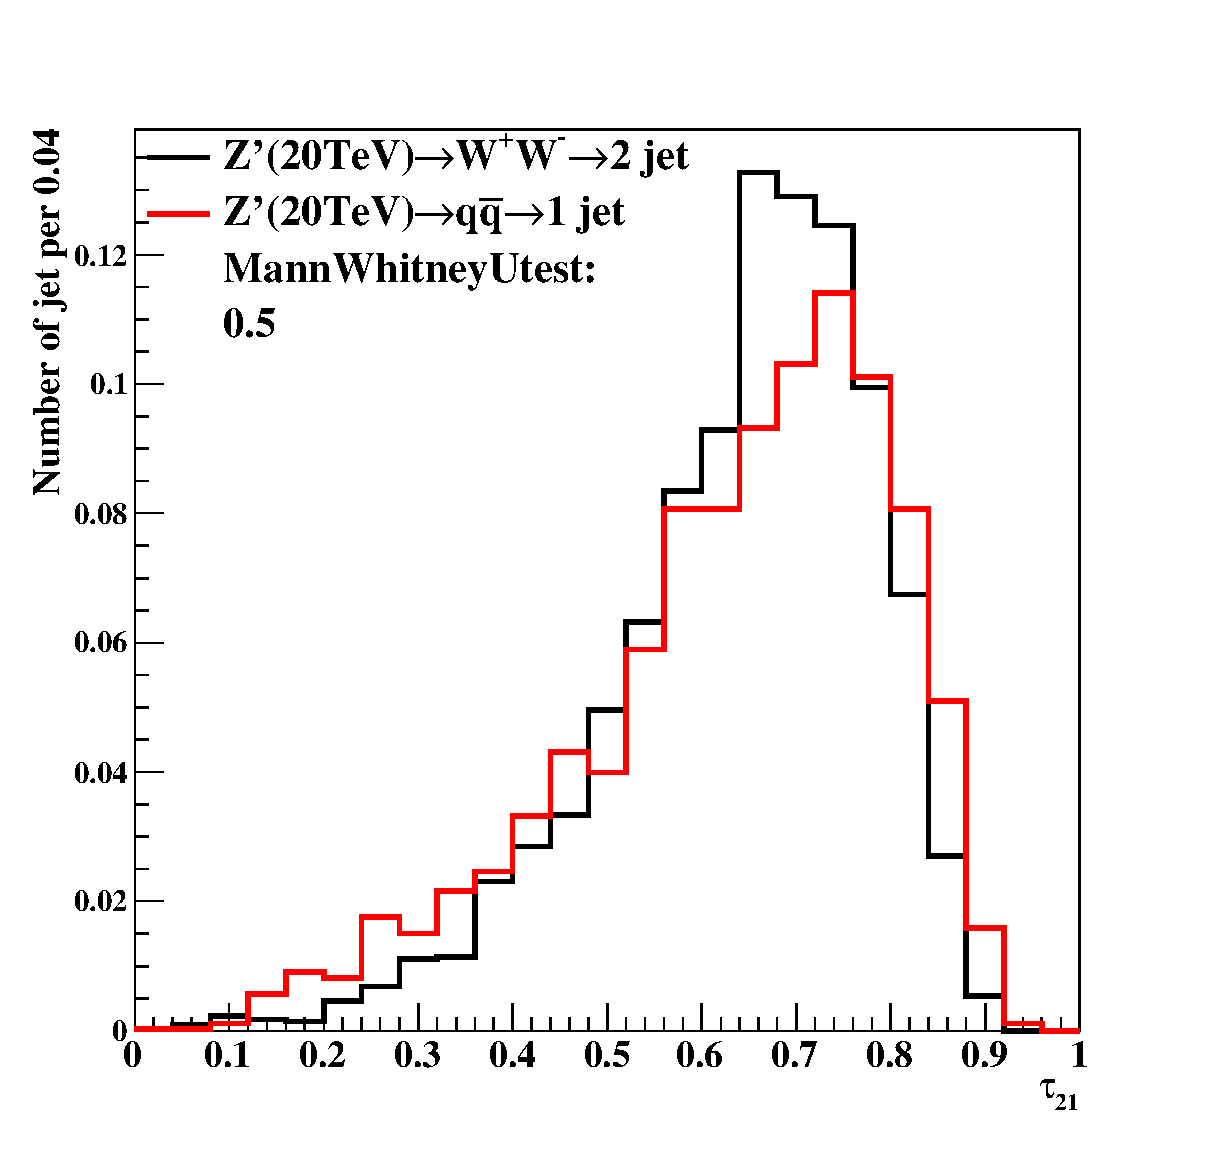
\includegraphics[width=0.43\textwidth]{figs/r009_tau21b1_20tev_04_U.eps}
   }
   \subfigure[5$\times$5(cm$\times$cm)] {
   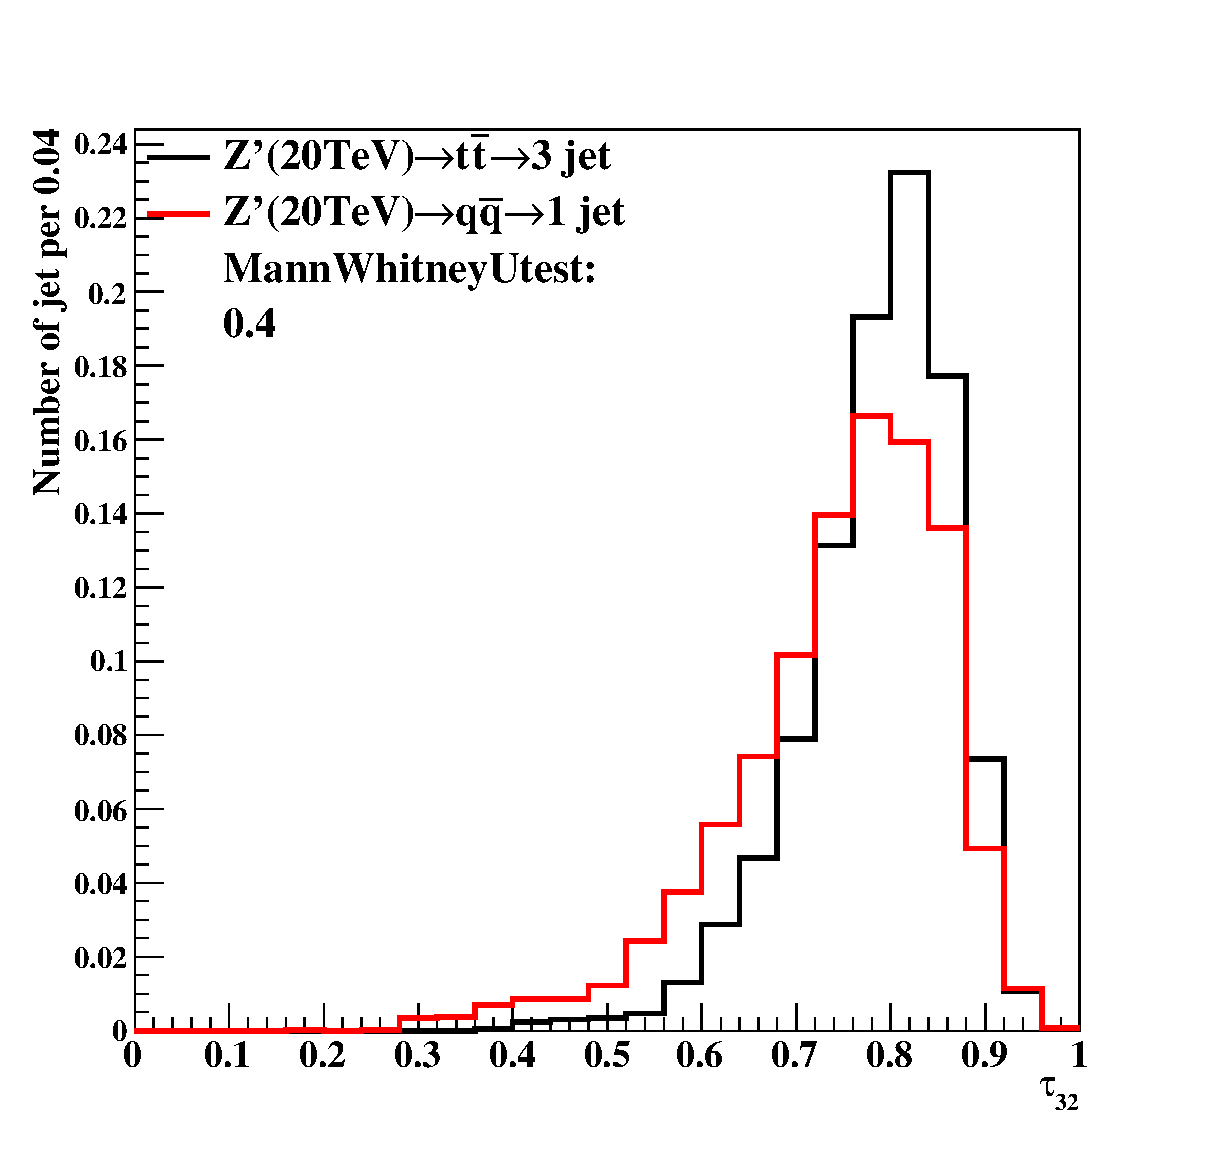
\includegraphics[width=0.43\textwidth]{figs/r009_tau32b1_20tev_04_U.eps}
   }
   \subfigure[1$\times$1(cm$\times$cm)] {
   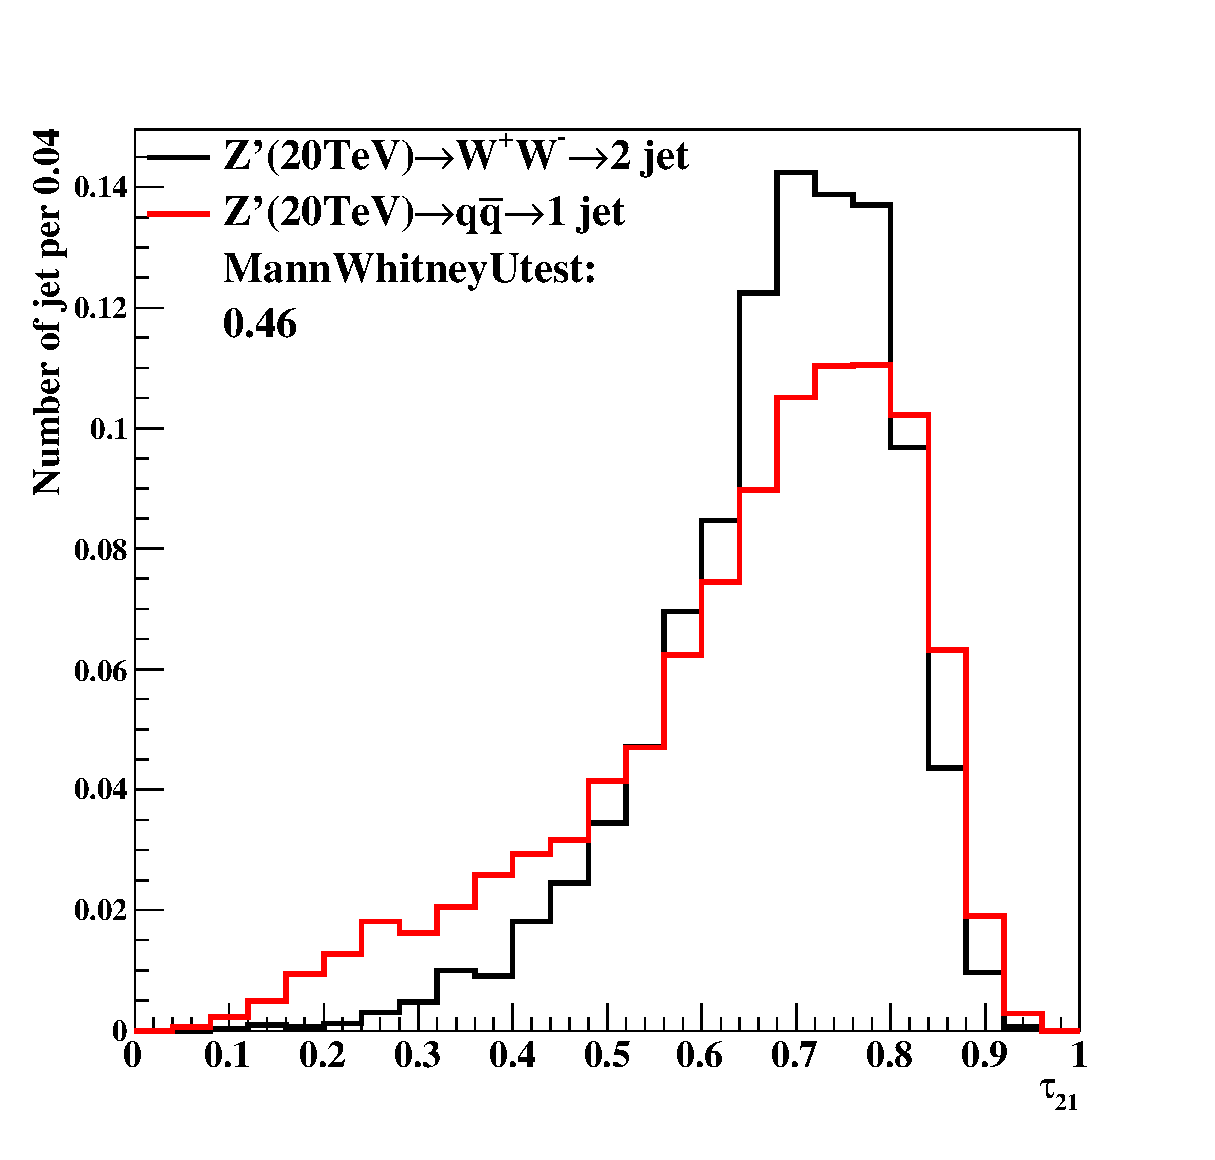
\includegraphics[width=0.43\textwidth]{figs/r012_tau21b1_20tev_04_U.eps}
   }
   \subfigure[1$\times$1(cm$\times$cm)] {
   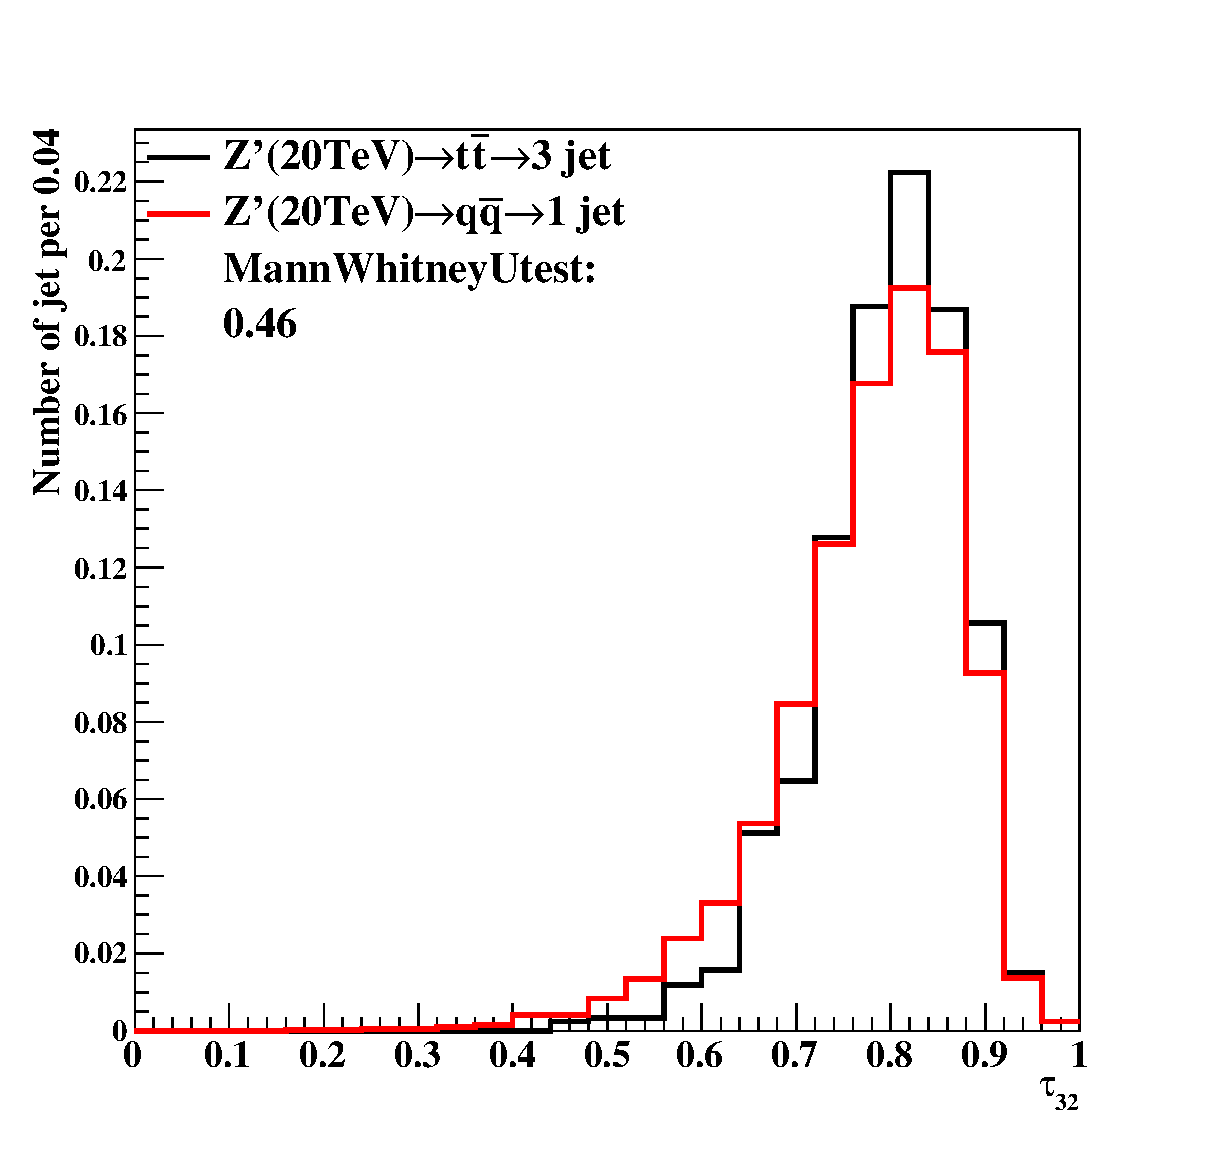
\includegraphics[width=0.43\textwidth]{figs/r012_tau32b1_20tev_04_U.eps}
   }

\end{center}
\caption{Distributions and U value in 20TeV energy collision for $\tau_{21}$,$\tau_{32}$ in different detector sizes. Cell Size in 20$\times$20,5$\times$5 and 1$\times$1(cm$\times$cm) are shown here.}
\label{fig:cluster_tau21_tau32}
\end{figure}


\begin{figure}
\begin{center}
   \subfigure[$\tau_{21}$] {
   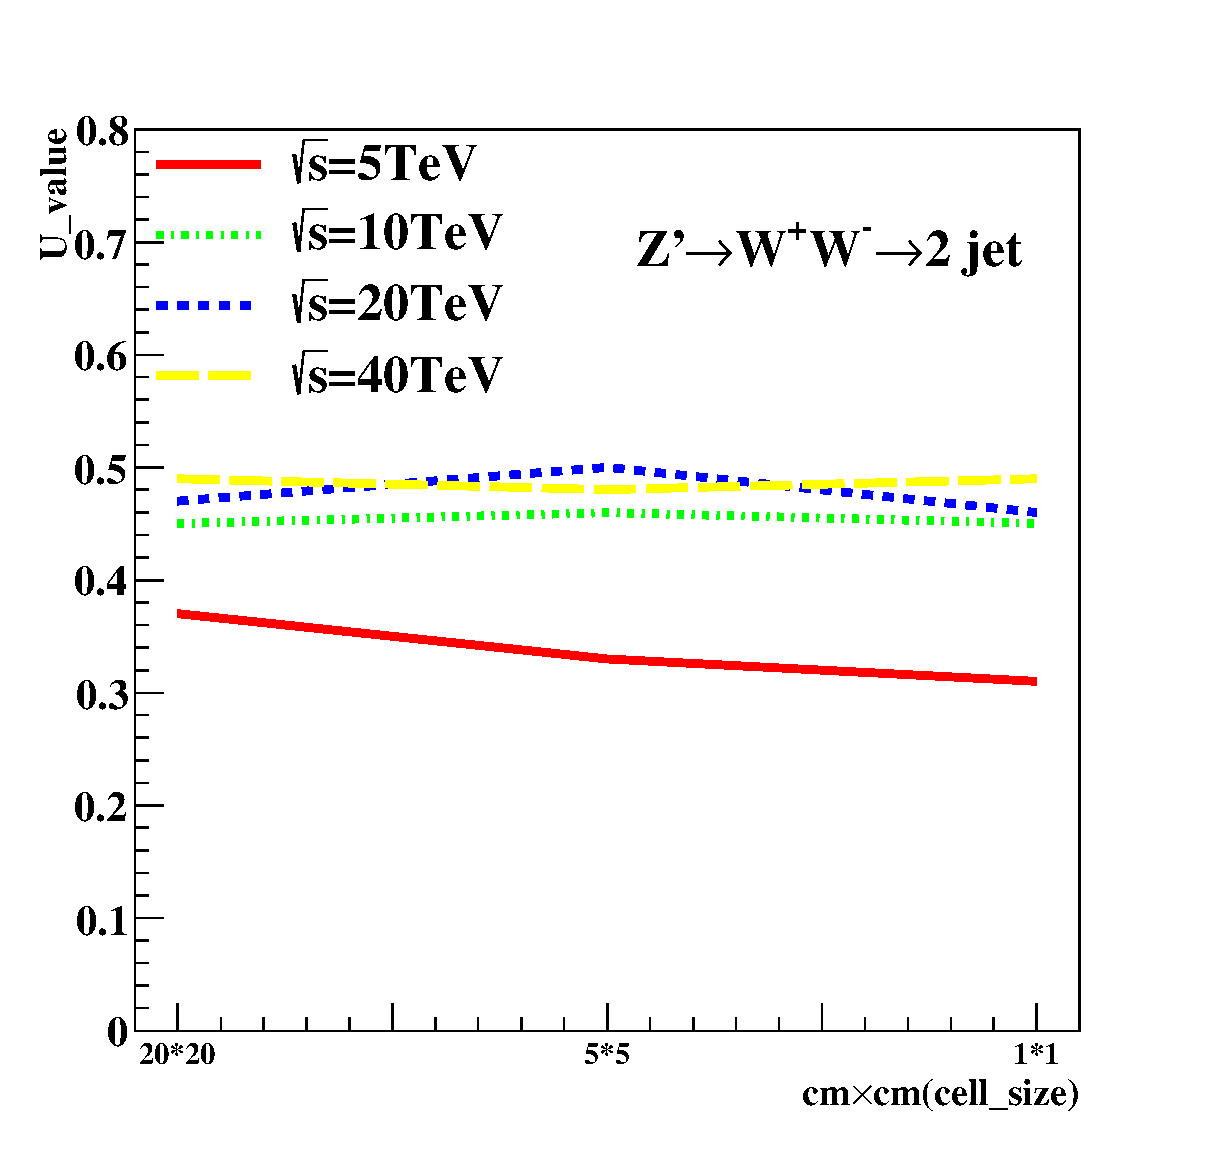
\includegraphics[width=0.43\textwidth]{figs/cluster_tau21_summary_U.eps}\hfill
   }
   \subfigure[$\tau_{32}$] {
   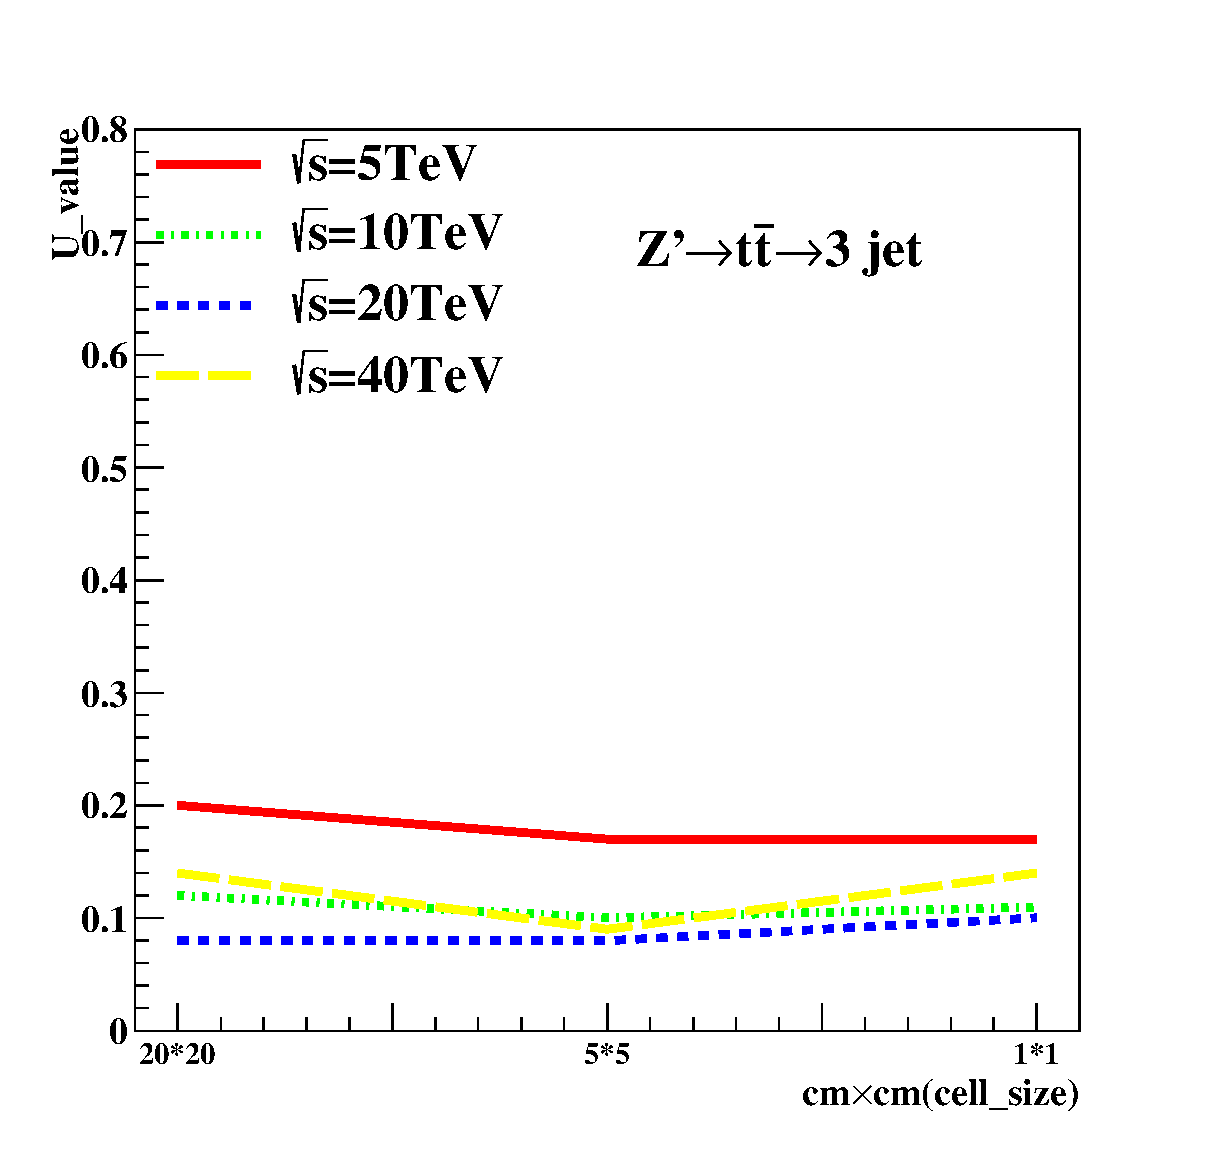
\includegraphics[width=0.43\textwidth]{figs/cluster_tau32_summary_U.eps}
   }
   \subfigure[$c_2^{(1)}$] {
   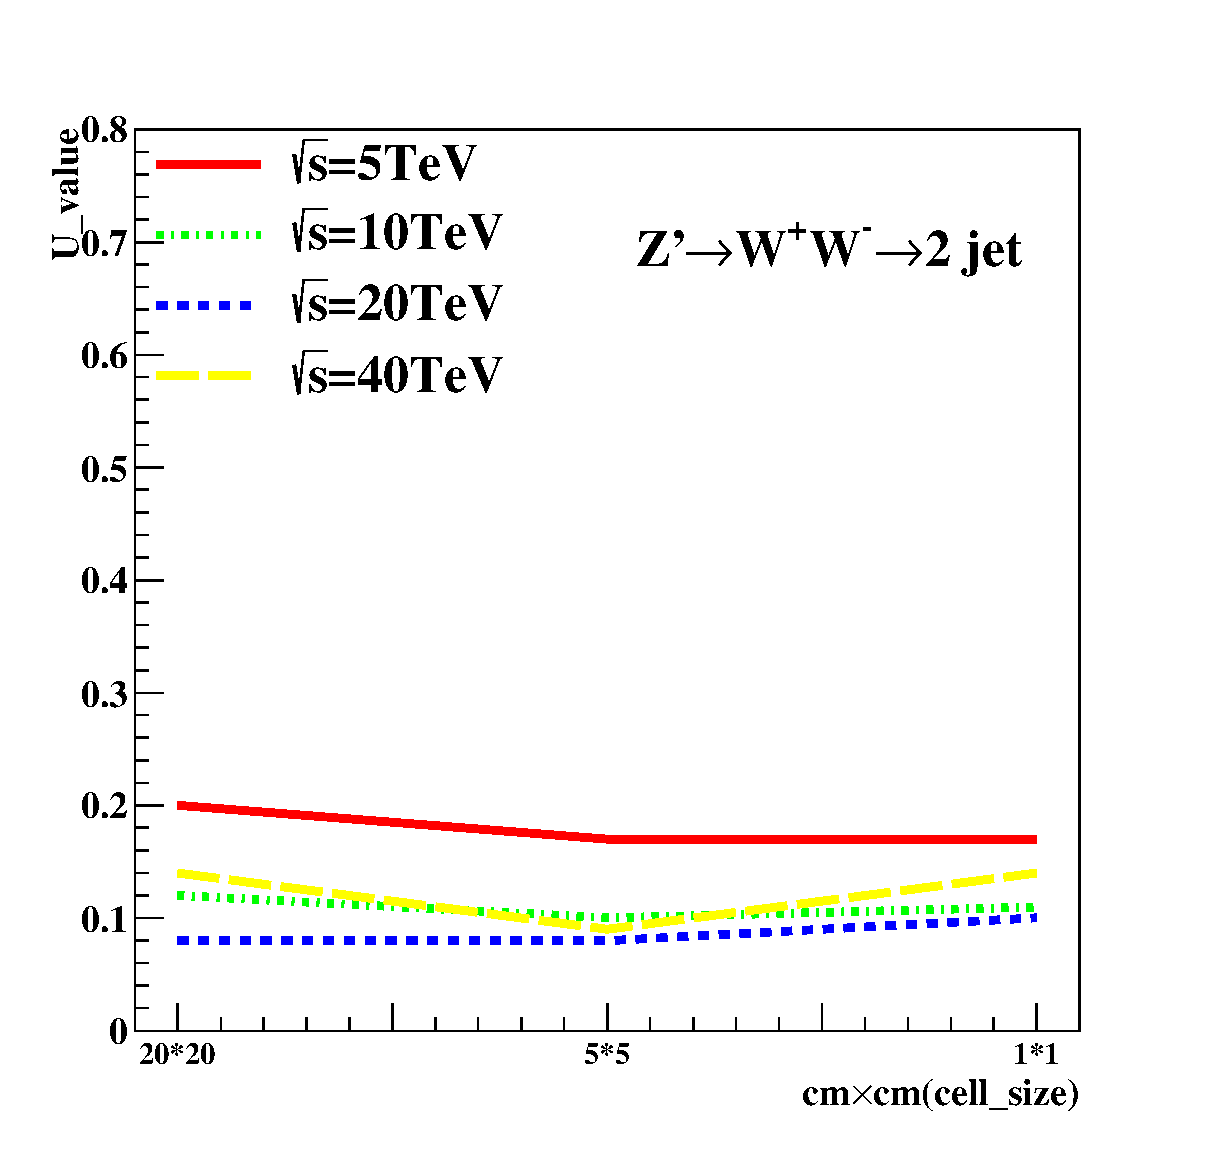
\includegraphics[width=0.43\textwidth]{figs/cluster_c2b1_summary_U.eps}
   }
\end{center}
\caption{U value for $\tau_{21}$,$\tau_{32}$ and $c_2^{(1)}$ at different collision energies correspond to different detector sizes in cluster. The energies of collision at 5, 10, 20, 40TeV are shown in each picture.}
\label{fig:cluster_U_summary}
\end{figure}


\begin{figure}
\begin{center}
   \subfigure[$\tau_{21}$] {
   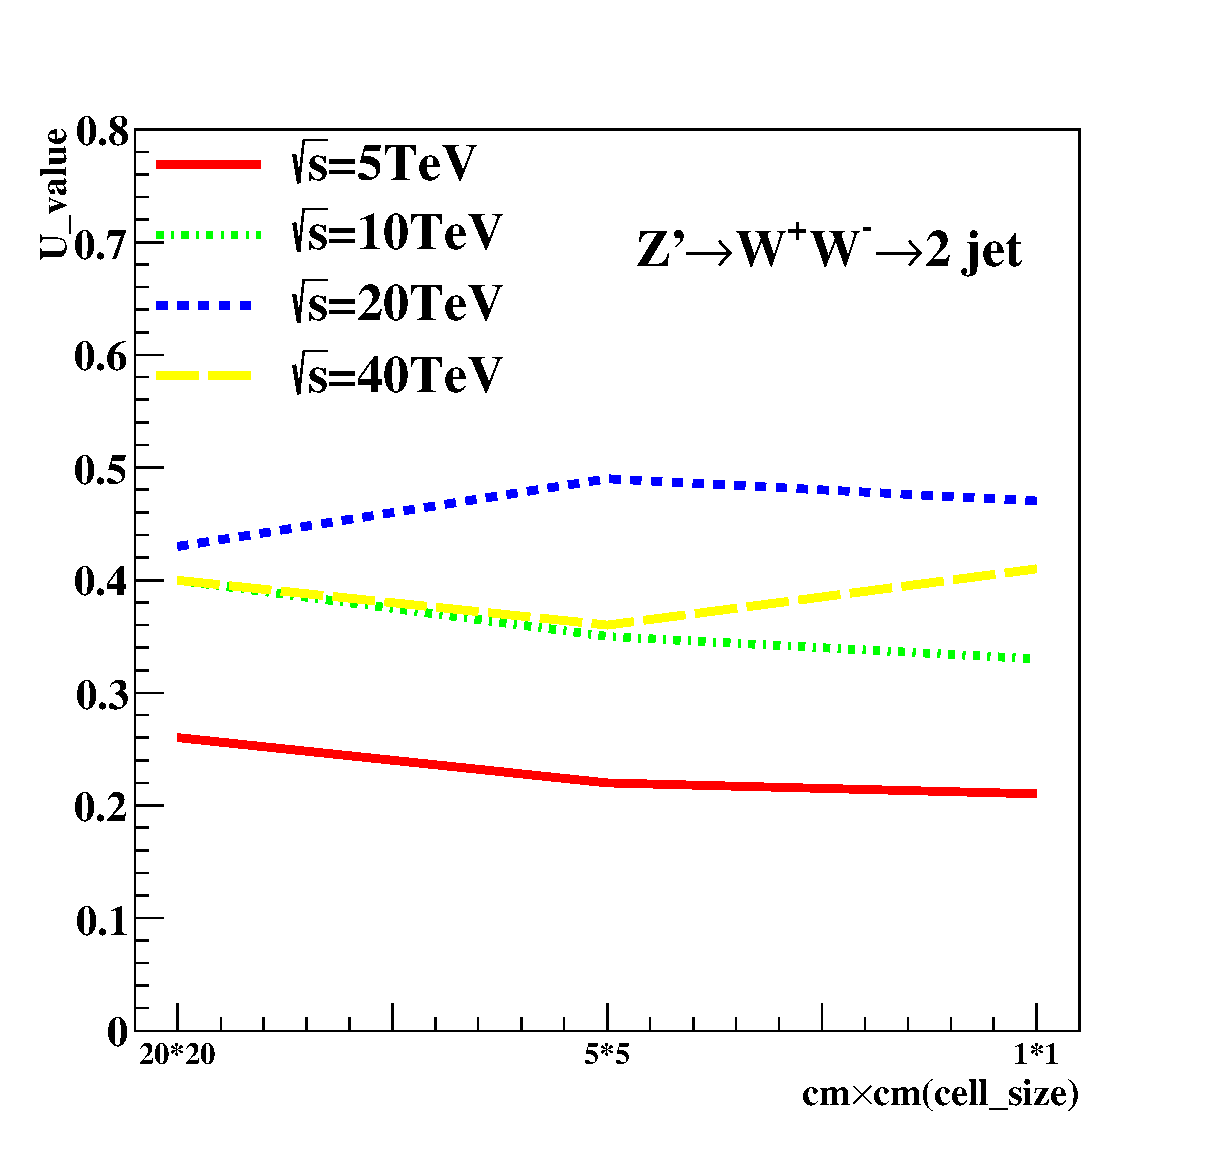
\includegraphics[width=0.43\textwidth]{figs/raw_tau21_summary_U.eps}\hfill
   }
   \subfigure[$\tau_{32}$] {
   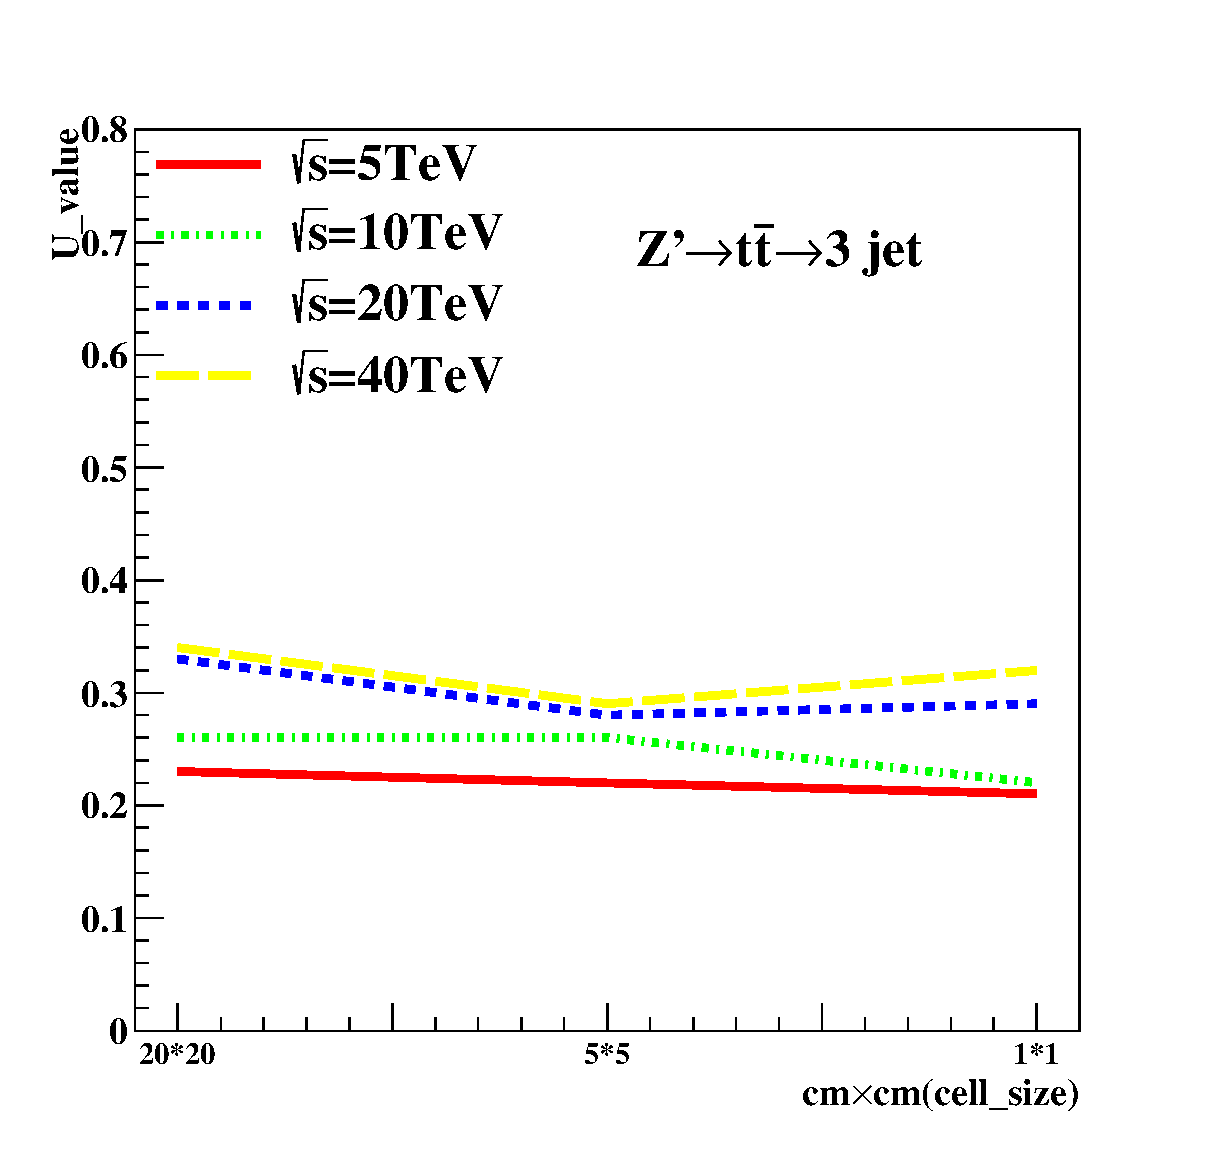
\includegraphics[width=0.43\textwidth]{figs/raw_tau32_summary_U.eps}
   }
   \subfigure[$c_2^{(1)}$] {
   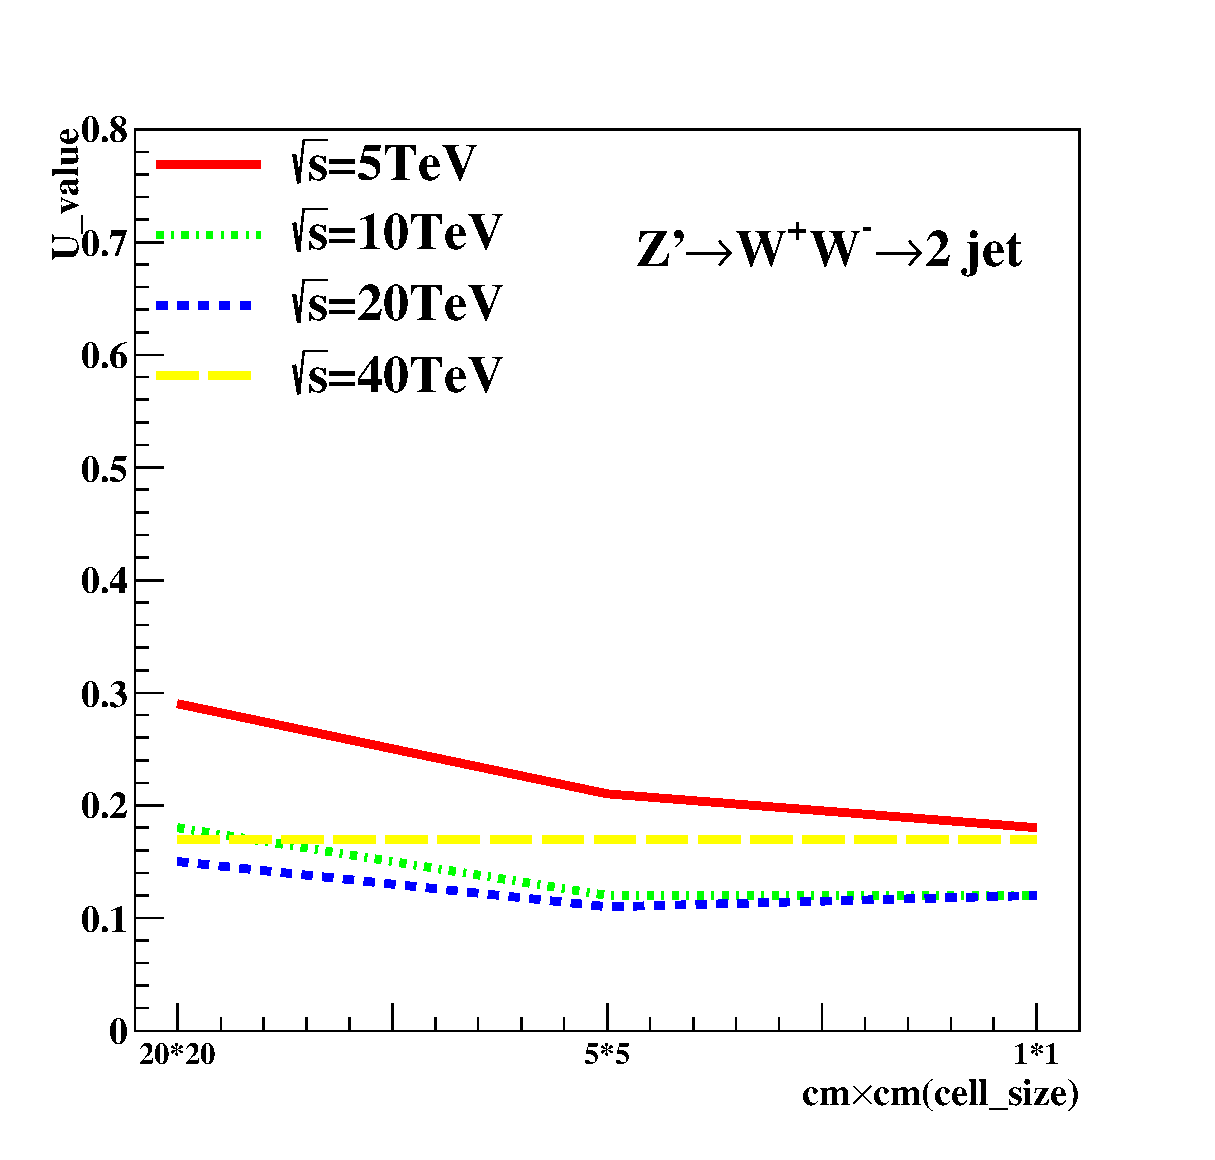
\includegraphics[width=0.43\textwidth]{figs/raw_c2b1_summary_U.eps}
   }
\end{center}
\caption{U value for $\tau_{21}$,$\tau_{32}$ and $c_2^{(1)}$ at different collision energies correspond to different detector sizes in rawhit cut at 0.5GeV. The energies of collision at 5, 10, 20, 40TeV are shown in each picture.}
\label{fig:raw_U_summary}
\end{figure}







\section*{Acknowledgements}
This research was performed using resources provided by the Open Science Grid,
which is supported by the National Science Foundation and the U.S. Department of Energy's Office of Science. 
We gratefully acknowledge the computing resources provided on Blues, 
a high-performance computing cluster operated by the Laboratory Computing Resource Center at Argonne National Laboratory.
Argonne National Laboratory's work was supported by the U.S. Department of Energy, Office of Science under contract DE-AC02-06CH11357.
The Fermi National Accelerator Laboratory (Fermilab) is operated by Fermi Research Alliance, LLC under Contract No. DE-AC02-07CH11359 with the United States Department of Energy.

\section*{Appendix}

\section*{Another study about the c variables}
In the past paper~\cite{Larkoski:2013eya}, It mention that in some process at $c_2$, when $\beta=1.7$, it will have the best separation power. We try to use this in our study to see whether it is suitable for our research.\\

In Figure \textcolor{blue}{9},\textcolor{blue}{1}0 and \textcolor{blue}{11}, they are the ROC curves of the different $\beta$ quantities in $c_2$ at different energies of collision. We can see that in all cell sizes, separation power isn't improved by increasing $\beta$ quantity to 1.7. We can see from $\beta=1$ to $\beta=2$, the separation power is worse and worse in all cell sizes in all energies of collision.\\
\label{sec:c_variables_study}

%1$\times$1(cm$\times$cm)
\begin{figure}
\begin{center}
   \subfigure[5TeV] {
   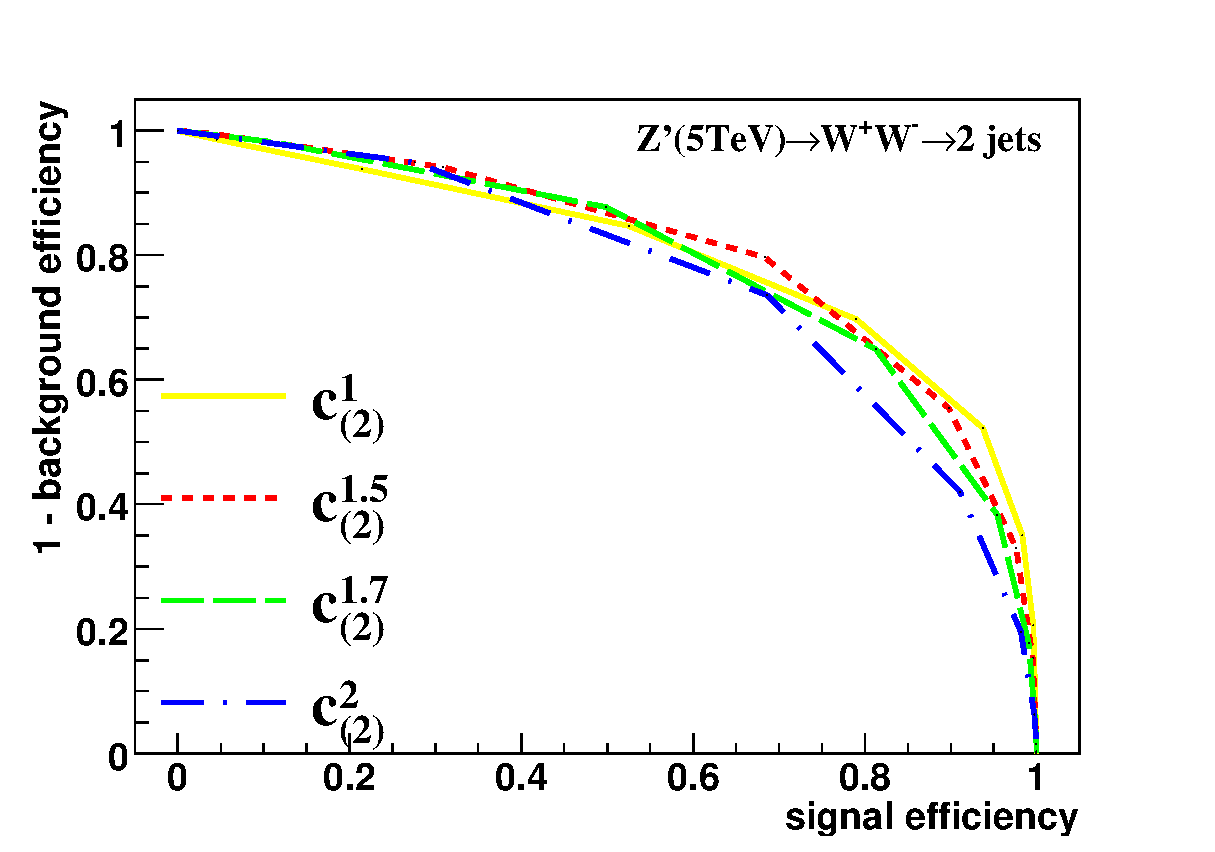
\includegraphics[width=0.43\textwidth]{figs/cluster_r010_c_variable_5tev_04_eff.eps}\hfill
   }
   \subfigure[10TeV] {
   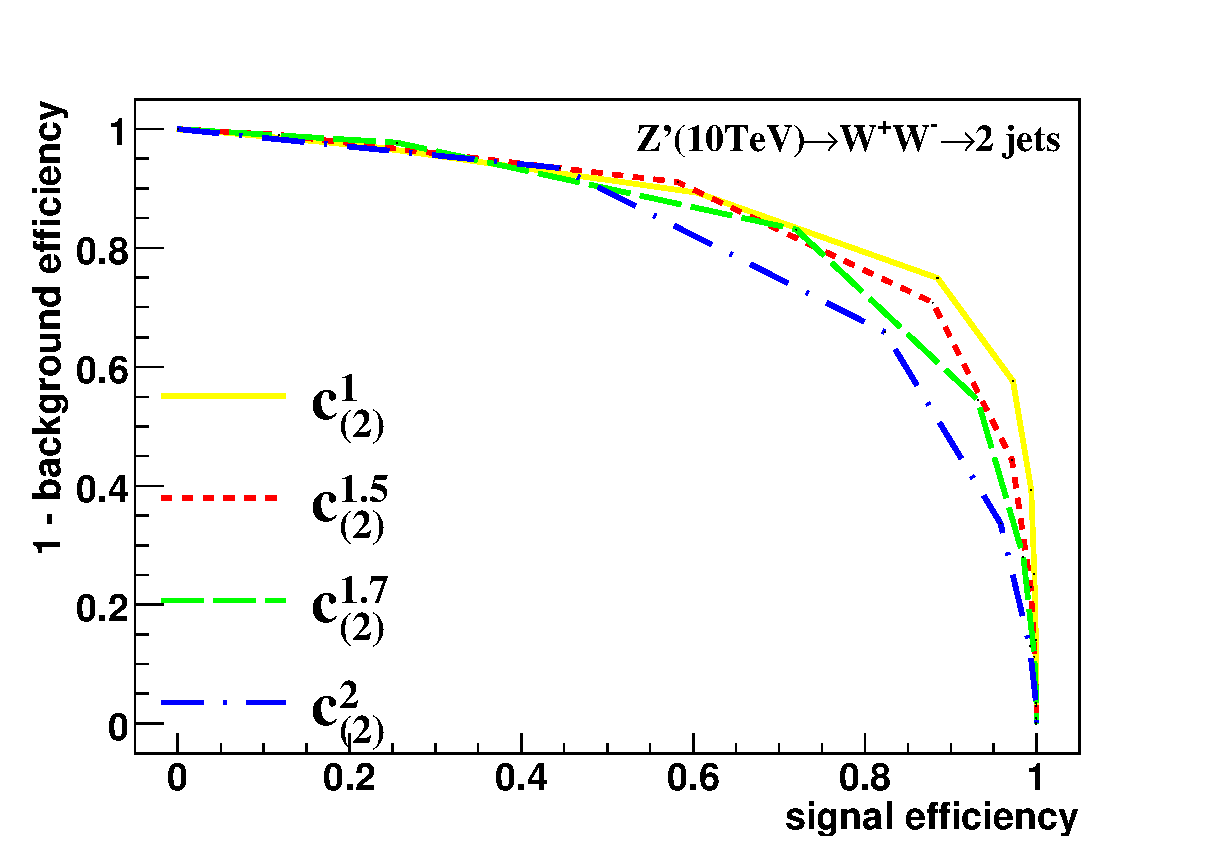
\includegraphics[width=0.43\textwidth]{figs/cluster_r010_c_variable_10tev_04_eff.eps}
   }
   \subfigure[20TeV] {
   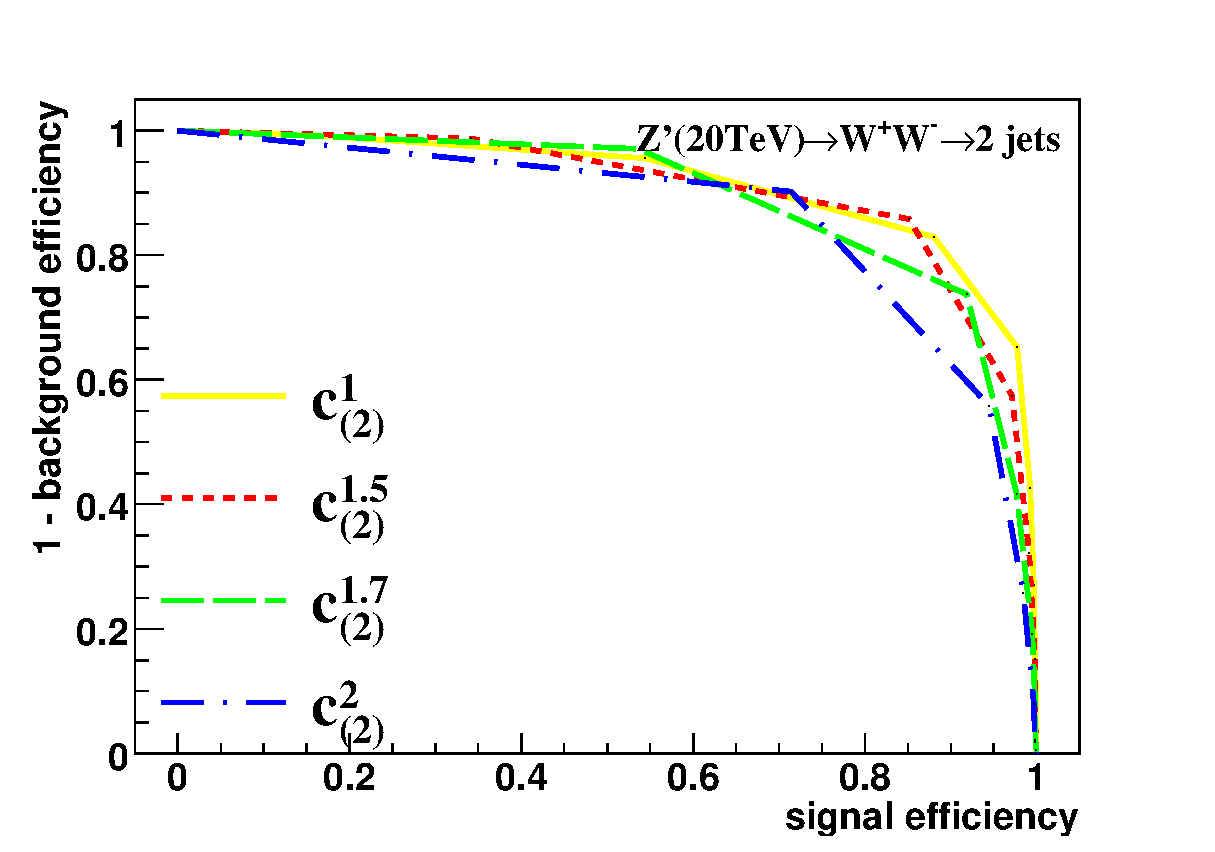
\includegraphics[width=0.43\textwidth]{figs/cluster_r010_c_variable_20tev_04_eff.eps}
   }
   \subfigure[40TeV] {
   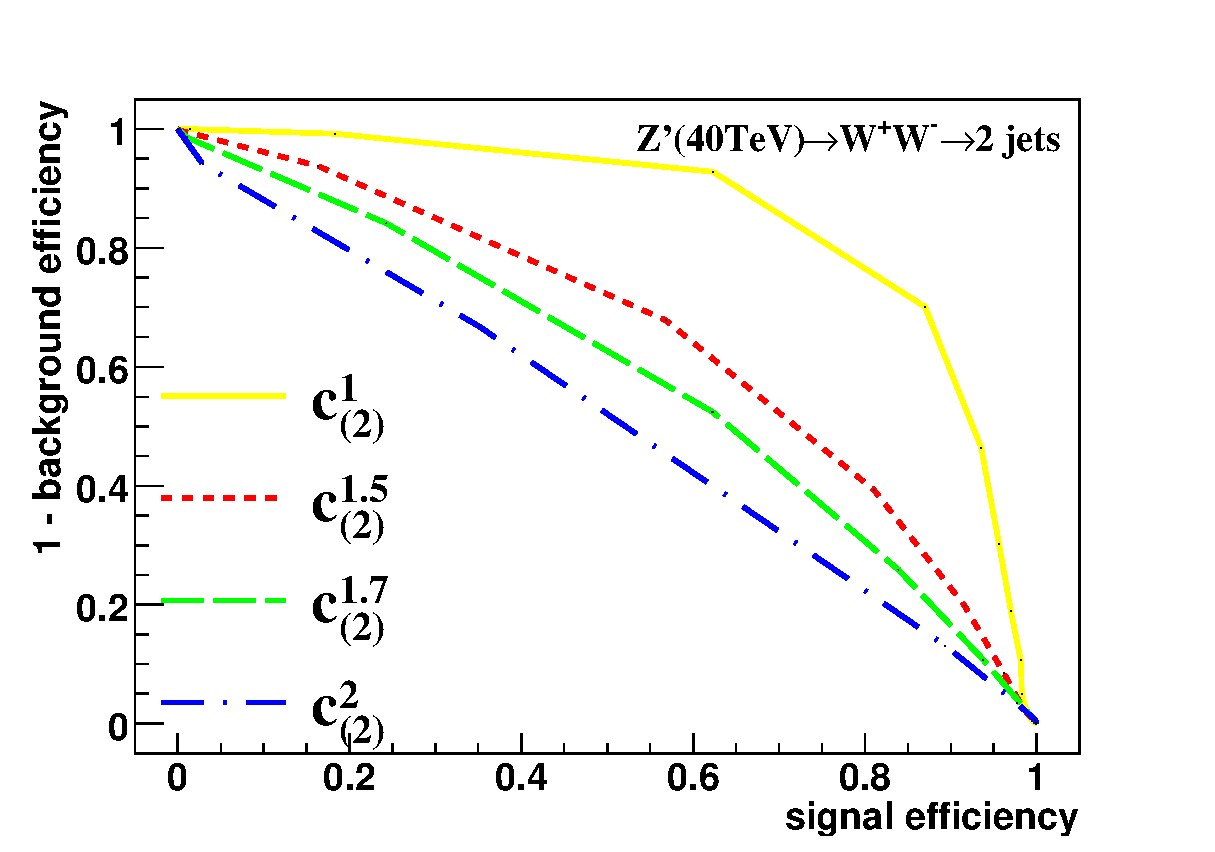
\includegraphics[width=0.43\textwidth]{figs/cluster_r010_c_variable_40tev_04_eff.eps}
   }

\end{center}
\caption{Signal efficiency versus background rejection rate using $c_2^{(1)}$,$c_2^{(1.5)}$,$c_2^{(1.7)}$,$c_2^{(2)}$ in different energies of collision for the cell size of  20$\times$20(cm$\times$cm).The energies of collision at (a)5, (b)10, (c)20, (d)40TeV are shown here.}
\label{fig:cluster_r010_c_variable}
\end{figure}

\begin{figure}
\begin{center}
   \subfigure[5TeV] {
   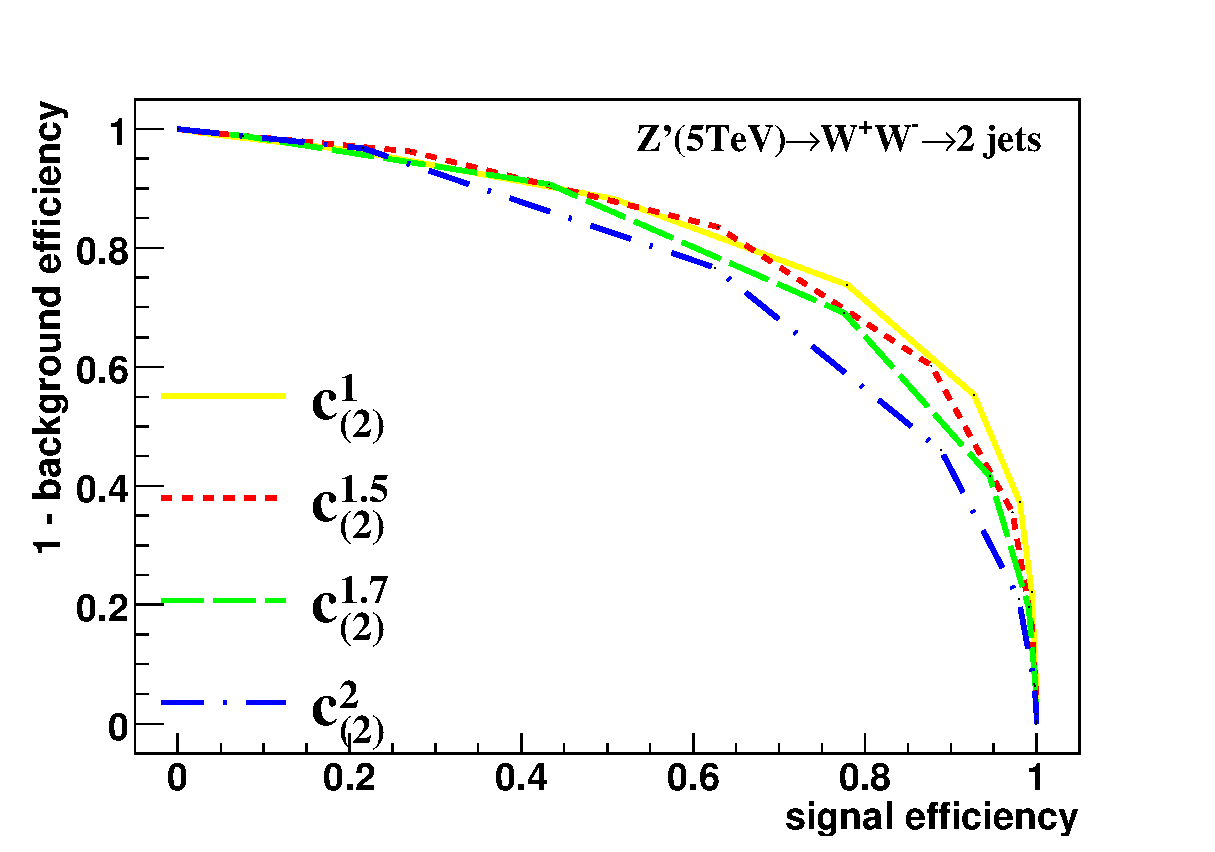
\includegraphics[width=0.43\textwidth]{figs/cluster_r009_c_variable_5tev_04_eff.eps}\hfill
   }
   \subfigure[10TeV] {
   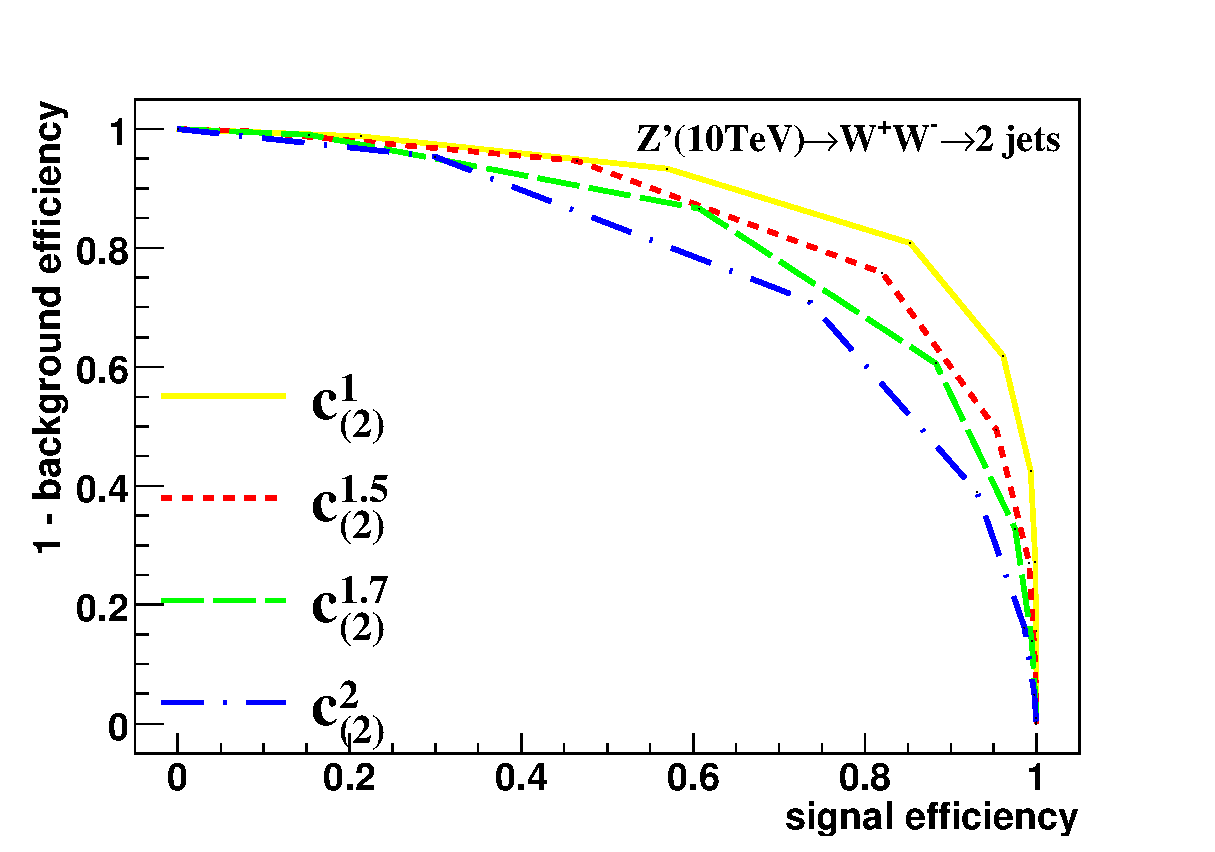
\includegraphics[width=0.43\textwidth]{figs/cluster_r009_c_variable_10tev_04_eff.eps}
   }
   \subfigure[20TeV] {
   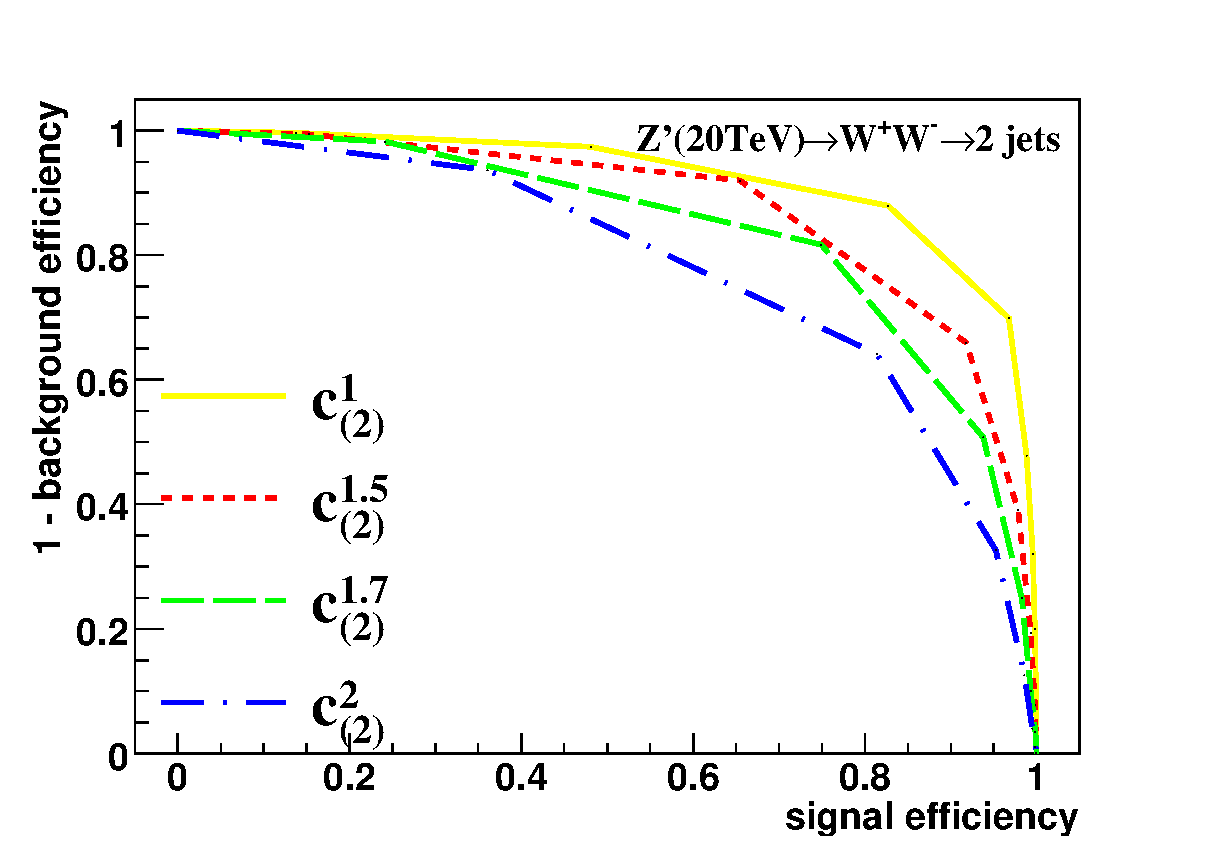
\includegraphics[width=0.43\textwidth]{figs/cluster_r009_c_variable_20tev_04_eff.eps}
   }
   \subfigure[40TeV] {
   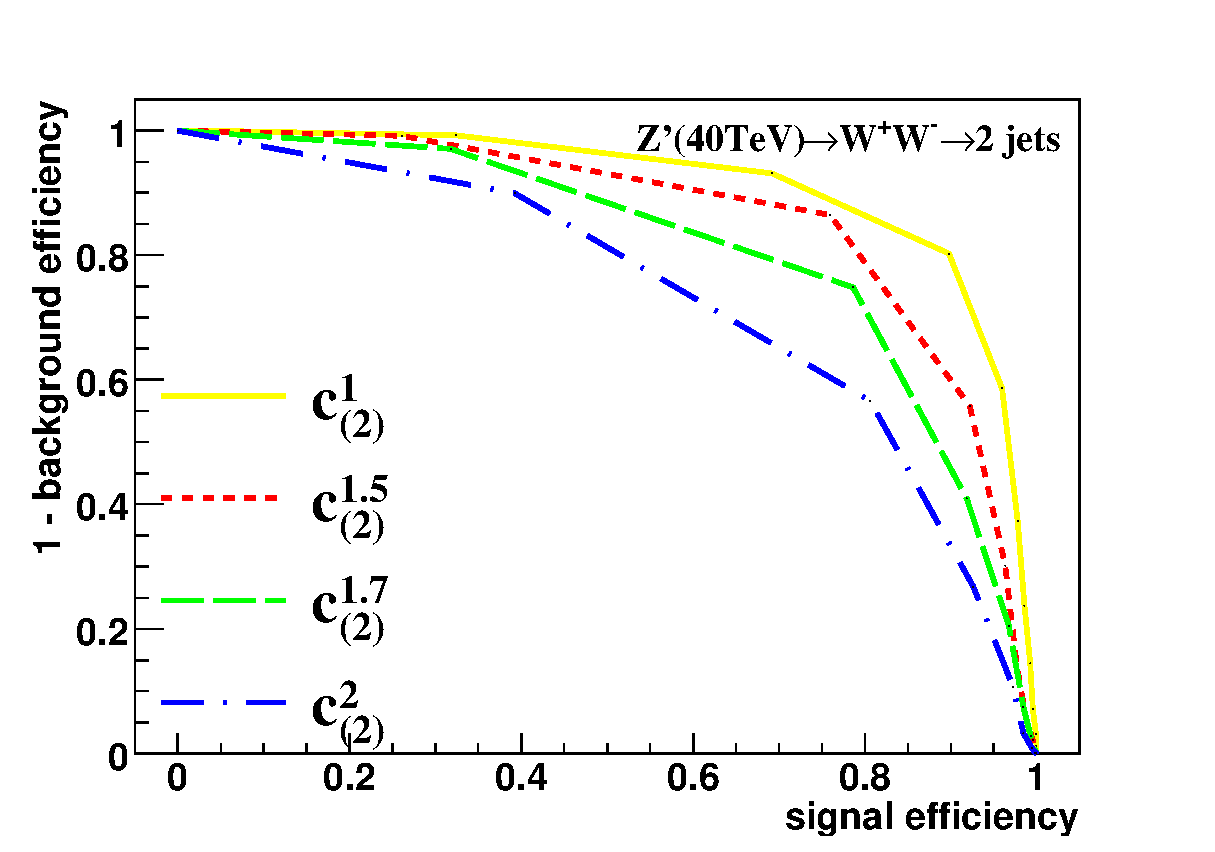
\includegraphics[width=0.43\textwidth]{figs/cluster_r009_c_variable_40tev_04_eff.eps}
   }

\end{center}
\caption{Signal efficiency versus background rejection rate using $c_2^{(1)}$,$c_2^{(1.5)}$,$c_2^{(1.7)}$,$c_2^{(2)}$ in different energies of collision for the cell size of  5$\times$5(cm$\times$cm).The energies of collision at (a)5, (b)10, (c)20, (d)40TeV are shown here.}
\label{cluster_r009_c_variable}
\end{figure}

\begin{figure}
\begin{center}
   \subfigure[5TeV] {
   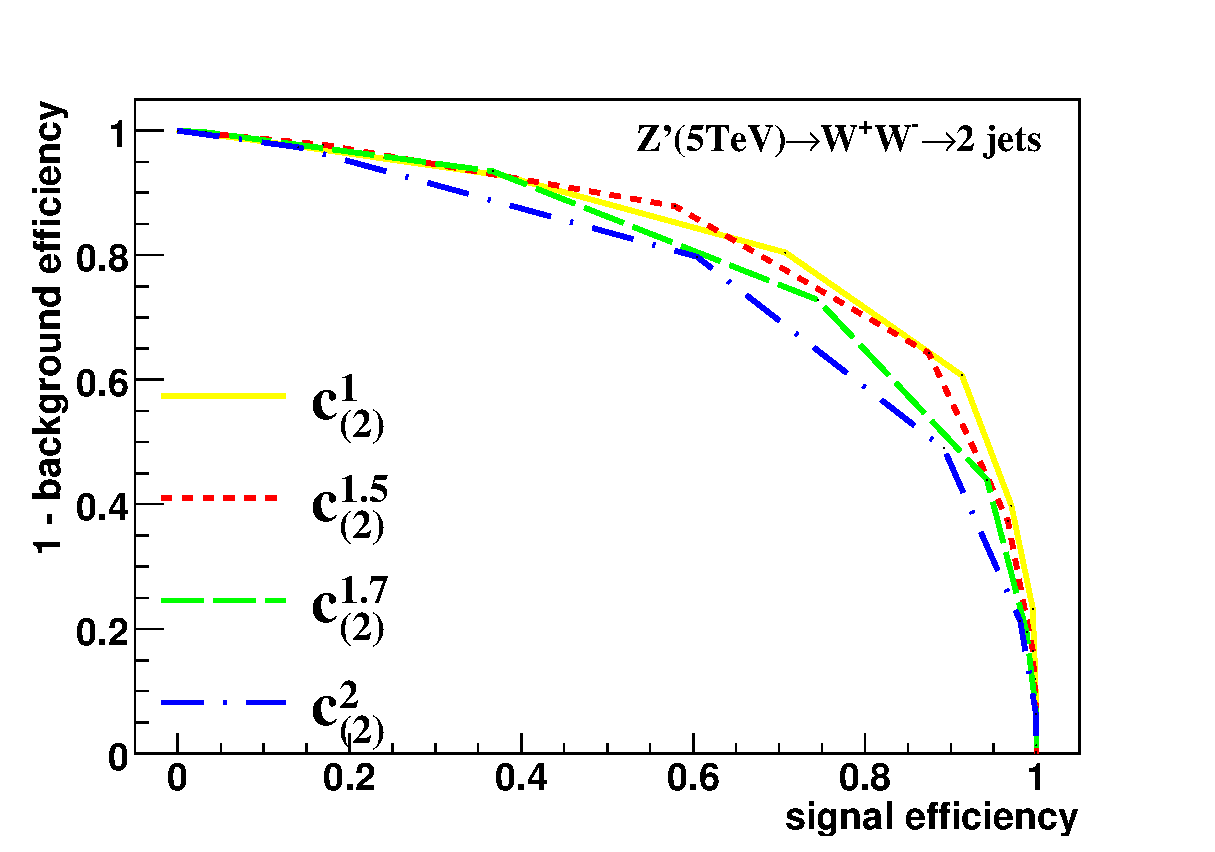
\includegraphics[width=0.43\textwidth]{figs/cluster_r012_c_variable_5tev_04_eff.eps}\hfill
   }
   \subfigure[10TeV] {
   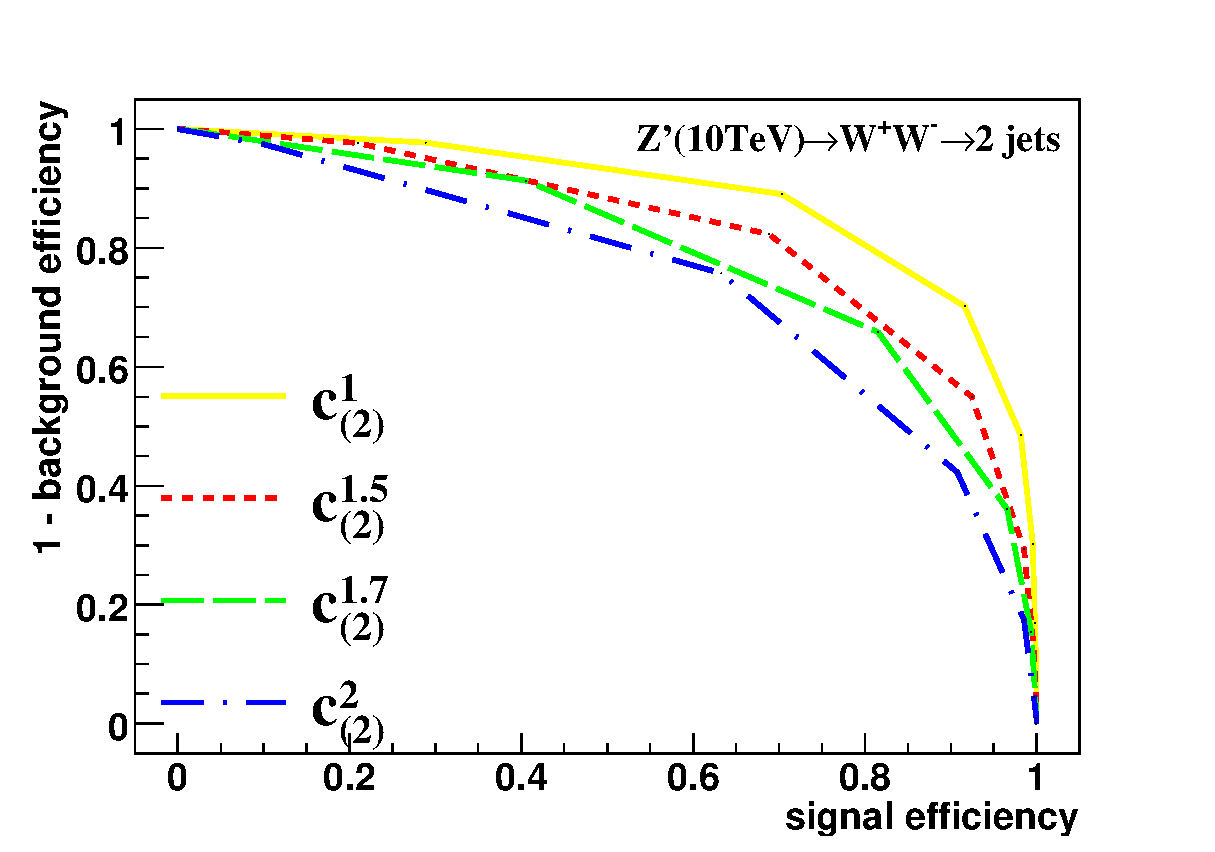
\includegraphics[width=0.43\textwidth]{figs/cluster_r012_c_variable_10tev_04_eff.eps}
   }
   \subfigure[20TeV] {
   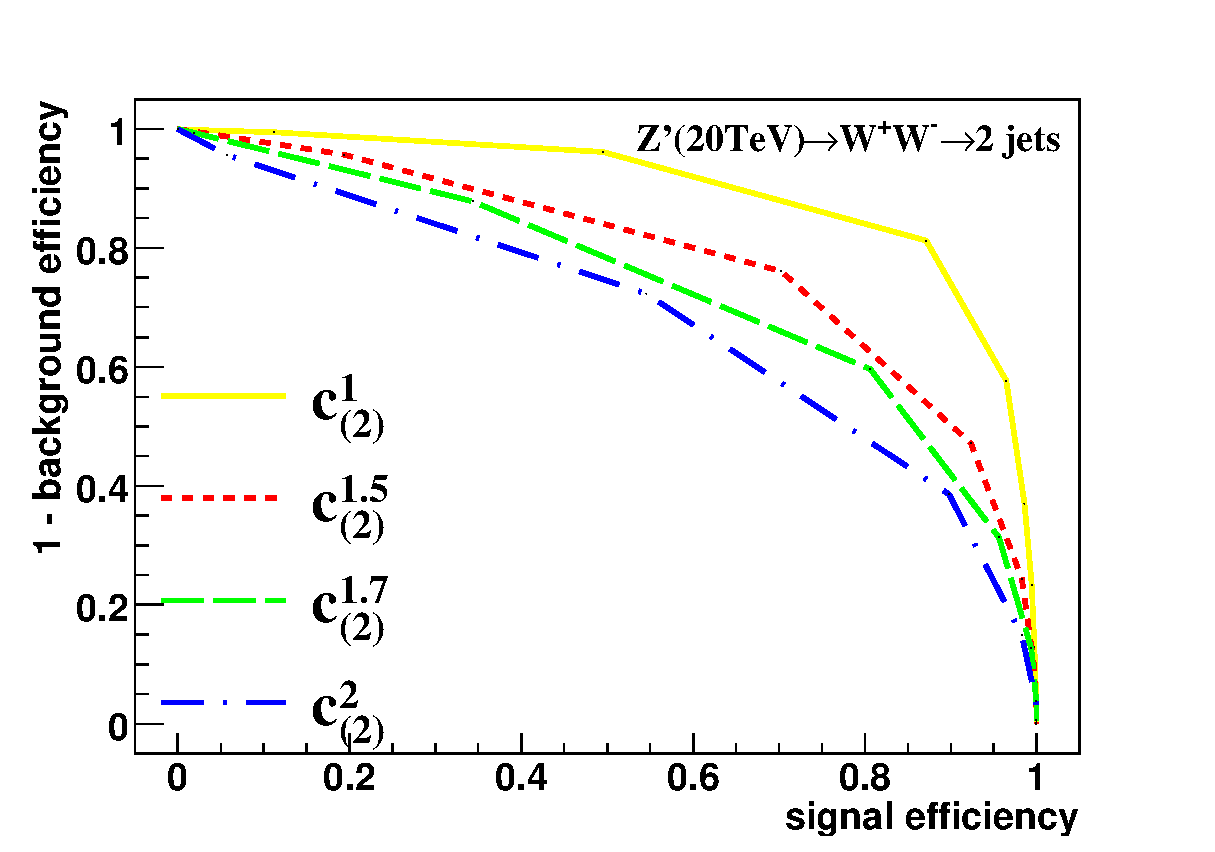
\includegraphics[width=0.43\textwidth]{figs/cluster_r012_c_variable_20tev_04_eff.eps}
   }
   \subfigure[40TeV] {
   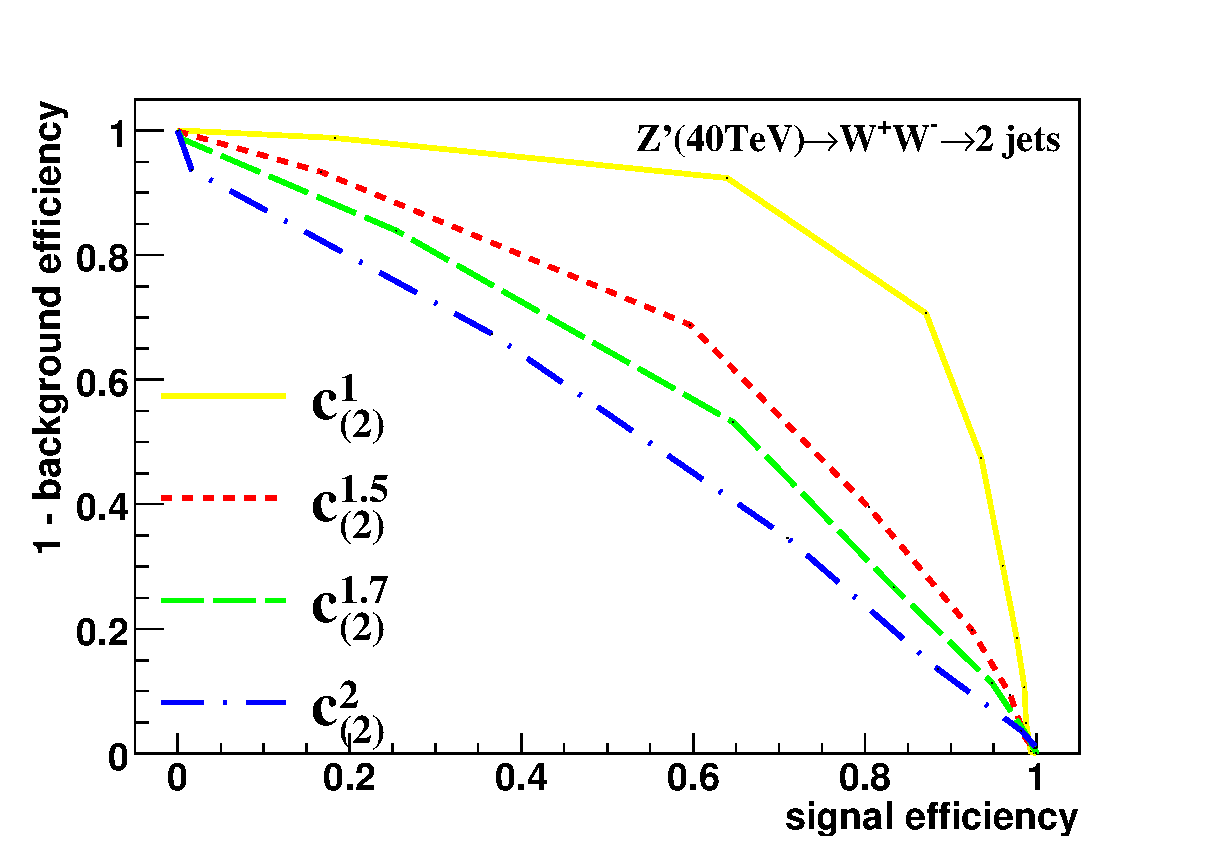
\includegraphics[width=0.43\textwidth]{figs/cluster_r012_c_variable_40tev_04_eff.eps}
   }

\end{center}
\caption{Signal efficiency versus background rejection rate using $c_2^{(1)}$,$c_2^{(1.5)}$,$c_2^{(1.7)}$,$c_2^{(2)}$ in different energies of collision for the cell size of  1$\times$1(cm$\times$cm).The energies of collision at (a)5, (b)10, (c)20, (d)40TeV are shown here.}
\label{cluster_r012_c_variable}
\end{figure}





\newpage
%%%%%%%%%%%%%%%%%%%%%% references %%%%%%%%%%%%%%%%%%%%%%%%%%%%%%
\section*{References}

\bibliographystyle{elsarticle-num}
\def\bibname{\Large\bf References}
\def\refname{\Large\bf References}
\pagestyle{plain}
\bibliography{biblio}



\end{document}
